% UCL Thesis LaTeX Template
%  (c) Ian Kirker, 2014
% 
% This is a template/skeleton for PhD/MPhil/MRes theses.
%
% It uses a rather split-up file structure because this tends to
%  work well for large, complex documents.
% We suggest using one file per chapter, but you may wish to use more
%  or fewer separate files than that.
% We've also separated out various bits of configuration into their
%  own files, to keep everything neat.
% Note that the \input command just streams in whatever file you give
%  it, while the \include command adds a page break, and does some
%  extra organisation to make compilation faster. Note that you can't
%  use \include inside an \include-d file.
% We suggest using \input for settings and configuration files that
%  you always want to use, and \include for each section of content.
% If you do that, it also means you can use the \includeonly statement
%  to only compile up the section you're currently interested in.
% You might also want to put figures into their own files to be \input.

% For more information on \input and \include, see:
%  http://tex.stackexchange.com/questions/246/when-should-i-use-input-vs-include


% Formatting rules for theses are here: 
%  http://www.ucl.ac.uk/current-students/research_degrees/thesis_formatting
% Binding and submitting guidelines are here:
%  http://www.ucl.ac.uk/current-students/research_degrees/thesis_binding_submission

% This package goes first and foremost, because it checks all 
%  your syntax for mistakes and some old-fashioned LaTeX commands.
% Note that normally you should load your documentclass before 
%  packages, because some packages change behaviour based on
%  your document settings.
% Also, for those confused by the RequirePackage here vs usepackage
%  elsewhere, usepackage cannot be used before the documentclass
%  command, while RequirePackage can. That's the only functional
%  difference.
\RequirePackage[l2tabu, orthodox]{nag}


% ------ Main document class specification ------
% The draft option here prevents images being inserted,
%  and adds chunky black bars to boxes that are exceeding 
%  the page width (to show that they are).
% The oneside option can optionally be replaced by twoside if
%  you intend to print double-sided. Note that this is
%  *specifically permitted* by the UCL thesis formatting
%  guidelines.
%
% Valid options in terms of type are:
%  phd
%  mres
%  mphil
%\documentclass[12pt,phd,draft,a4paper,oneside]{ucl_thesis}
\documentclass[12pt,phd,a4paper,oneside]{ucl_thesis}
\usepackage{enumerate}
\usepackage{algorithm}
\usepackage{algpseudocode}

% Package configuration:
%  LaTeX uses "packages" to add extra commands and features.
%  There are quite a few useful ones, so we've put them in a 
%   separate file.
% -------- Packages --------

% This package just gives you a quick way to dump in some sample text.
% You can remove it -- it's just here for the examples.
\usepackage{blindtext}

% This package means empty pages (pages with no text) won't get stuff
%  like chapter names at the top of the page. It's mostly cosmetic.
\usepackage{emptypage}

% The graphicx package adds the \includegraphics command,
%  which is your basic command for adding a picture.
\usepackage{graphicx}

% This command is provided by the graphicx package, and 
%  controls the default dpi resolution of images you use.
%  72 is the default, but 300 is more normal, and 600 is
%  as good as you can expect to be able to get on normal paper.
\pdfimageresolution=300


% The float package improves LaTeX's handling of floats,
%  and also adds the option to *force* LaTeX to put the float
%  HERE, with the [H] option to the float environment.
\usepackage{float}

% The amsmath package enhances the various ways of including
%  maths, including adding the align environment for aligned
%  equations.
\usepackage{amsmath}

% Use these two packages together -- they define symbols
%  for e.g. units that you can use in both text and math mode.
\usepackage{gensymb}
\usepackage{textcomp}
% You may also want the units package for making little
%  fractions for unit specifications.
%\usepackage{units}


% The setspace package lets you use 1.5-sized or double line spacing.
\usepackage{setspace}
\setstretch{1.5}

% That just does body text -- if you want to expand *everything*,
%  including footnotes and tables, use this instead:
%\renewcommand{\baselinestretch}{1.5}


% PGFPlots is either a really clunky or really good way to add graphs
%  into your document, depending on your point of view.
% There's waaaaay too much information on using this to cover here,
%  so, you might want to start here:
%   http://pgfplots.sourceforge.net/
%  or here:
%   http://pgfplots.sourceforge.net/pgfplots.pdf
%\usepackage{pgfplots}
%\pgfplotsset{compat=1.3} % <- this fixed axis labels in the version I was using

% PGFPlotsTable can help you make tables a little more easily than
%  usual in LaTeX.
% If you're going to have to paste data in a lot, I'd suggest using it.
%  You might want to start with the manual, here:
%  http://pgfplots.sourceforge.net/pgfplotstable.pdf
%\usepackage{pgfplotstable}

% These settings are also recommended for using with pgfplotstable.
%\pgfplotstableset{
%	% these columns/<colname>/.style={<options>} things define a style
%	% which applies to <colname> only.
%	empty cells with={--}, % replace empty cells with '--'
%	every head row/.style={before row=\toprule,after row=\midrule},
%	every last row/.style={after row=\bottomrule}
%}


% The mhchem package provides chemistry formula typesetting commands
%  e.g. \ce{H2O}
%\usepackage[version=3]{mhchem}

% And the chemfig package gives a weird command for adding Lewis 
%  diagrams, for e.g. organic molecules
%\usepackage{chemfig}

% The linenumbers command from the lineno package adds line numbers
%  alongside your text that can be useful for discussing edits 
%  in drafts.
% Remove or comment out the command for proper versions.
%\usepackage[modulo]{lineno}
% \linenumbers 


% Alternatively, you can use the ifdraft package to let you add
%  commands that will only be used in draft versions
%\usepackage{ifdraft}

% For example, the following adds a watermark if the draft mode is on.
%\ifdraft{
%  \usepackage{draftwatermark}
%  \SetWatermarkText{\shortstack{\textsc{Draft Mode}\\ \strut \\ \strut \\ \strut}}
%  \SetWatermarkScale{0.5}
%  \SetWatermarkAngle{90}
%}


% The multirow package adds the option to make cells span 
%  rows in tables.
\usepackage{multirow}


% Subfig allows you to create figures within figures, to, for example,
%  make a single figure with 4 individually labeled and referenceable
%  sub-figures.
% It's quite fiddly to use, so check the documentation.
%\usepackage{subfig}

% The natbib package allows book-type citations commonly used in
%  longer works, and less commonly in science articles (IME).
% e.g. (Saucer et al., 1993) rather than [1]
% More details are here: http://merkel.zoneo.net/Latex/natbib.php
%\usepackage{natbib}

% The bibentry package (along with the \nobibliography* command)
%  allows putting full reference lines inline.
%  See: 
%   http://tex.stackexchange.com/questions/2905/how-can-i-list-references-from-bibtex-file-in-line-with-commentary
\usepackage{bibentry} 

% The isorot package allows you to put things sideways 
%  (or indeed, at any angle) on a page.
% This can be useful for wide graphs or other figures.
%\usepackage{isorot}

% The caption package adds more options for caption formatting.
% This set-up makes hanging labels, makes the caption text smaller
%  than the body text, and makes the label bold.
% Highly recommended.
\usepackage[format=hang,font=small,labelfont=bf]{caption}

% If you're getting into defining your own commands, you might want
%  to check out the etoolbox package -- it defines a few commands
%  that can make it easier to make commands robust.
\usepackage{etoolbox}


% Sets up links within your document, for e.g. contents page entries
%  and references, and also PDF metadata.
% You should edit this!
%%
%% This file uses the hyperref package to make your thesis have metadata embedded in the PDF, 
%%  and also adds links to be able to click on references and contents page entries to go to 
%%  the pages.
%%

% Some hacks are necessary to make bibentry and hyperref play nicely.
% See: http://tex.stackexchange.com/questions/65348/clash-between-bibentry-and-hyperref-with-bibstyle-elsart-harv
\usepackage{bibentry}
\makeatletter\let\saved@bibitem\@bibitem\makeatother
\usepackage[pdftex,hidelinks]{hyperref}
\makeatletter\let\@bibitem\saved@bibitem\makeatother
\makeatletter
\AtBeginDocument{
    \hypersetup{
        pdfsubject={Thesis Subject},
        pdfkeywords={Thesis Keywords},
        pdfauthor={Author},
        pdftitle={Title},
    }
}
\makeatother
    


% And then some settings in separate files.
% These settings are from:
%  http://mintaka.sdsu.edu/GF/bibliog/latex/floats.html

% They give LaTeX more options on where to put your figures, and may
%  mean that fewer of your figures end up at the tops of pages far
%  away from the thing they're related to.

% Alters some LaTeX defaults for better treatment of figures:
% See p.105 of "TeX Unbound" for suggested values.
% See pp. 199-200 of Lamport's "LaTeX" book for details.

%   General parameters, for ALL pages:
\renewcommand{\topfraction}{0.9}	% max fraction of floats at top
\renewcommand{\bottomfraction}{0.8}	% max fraction of floats at bottom

%   Parameters for TEXT pages (not float pages):
\setcounter{topnumber}{2}
\setcounter{bottomnumber}{2}
\setcounter{totalnumber}{4}     % 2 may work better
\setcounter{dbltopnumber}{2}    % for 2-column pages
\renewcommand{\dbltopfraction}{0.9}	% fit big float above 2-col. text
\renewcommand{\textfraction}{0.07}	% allow minimal text w. figs

%   Parameters for FLOAT pages (not text pages):
\renewcommand{\floatpagefraction}{0.7}	% require fuller float pages
% N.B.: floatpagefraction MUST be less than topfraction !!
\renewcommand{\dblfloatpagefraction}{0.7}	% require fuller float pages

% remember to use [htp] or [htpb] for placement,
% e.g. 
%  \begin{figure}[htp]
%   ...
%  \end{figure} % For things like figures and tables
\bibliographystyle{unsrt}   % For bibliographies

% Title Settings
\setcounter{secnumdepth}{3}
\setcounter{tocdepth}{3}
\title{Transfer Thesis}
\author{Noradila Nordin}
\department{Department of Electronic \& Electrical Engineering}


\begin{document}



\nobibliography*
% This is a dumb trick that works with the bibentry package to let
%  you put bibliography entries whereever you like.
% I used this to put references to papers a chapter's work was 
%  published in at the end of that chapter.
% For more information, see: http://stefaanlippens.net/bibentry

% If you haven't finished making your full BibTex file yet, you
%  might find this useful -- it'll just replace all your
%  citations with little superscript notes.
% Uncomment to use.
%\renewcommand{\cite}[1]{\emph{\textsuperscript{[#1]}}}

% At last, content! Remember filenames are case-sensitive and 
%  *must not* include spaces.
\maketitle
\makedeclaration

\begin{abstract} % 300 word limit
%My research is about stuff.
%It begins with a study of some stuff, and then some other stuff and things.
%There is a 300-word limit on your abstract.

This report presents the current state of research work that has been carried out in the context of the PhD. (describe why do it). The PhD work proposes a new decentralised multi-channel tree building protocol with a centralised controller for ad-hoc sensor networks. The protocol alleviates the effect of interference which results in improved network efficiency and stability, and link reliability. The proposed protocol takes into account all available channels to utilise the spectrum and aims to use the spectrum efficiently by transmitting on several channels. The protocol detects which channels suffer interference and changes away from those channels. The algorithm for channel selection is a two-hop colouring protocol that reduces the chances of nearby nodes to transmit on the same channel. All nodes are battery operated except for the low power border router (LPBR). This enables a centralised channel switching process at the LPBR. The protocol is built based on the routing protocol for low power and lossy networks (RPL). In its initial phase, the protocol uses RPL's standard topology formation to create an initial working topology and then seeks to improve this topology by switching channels. The report discusses the main engineering and research challenges raised by the protocol, and describes and explains the principles and mechanisms used to support the proposed protocol. It then presents an extensive evaluation of the protocol and other other approaches. The implementation and evaluation of the protocol is performed using the Contiki framework. The report then describes the future main research issues that will be investigated in the context of this PhD.



In this report,

The proposed approach
The report discusses 
\end{abstract}

\begin{acknowledgements}
Acknowledge all the things!
\end{acknowledgements}

\setcounter{tocdepth}{2} 
% Setting this higher means you get contents entries for
%  more minor section headers.

\tableofcontents
\listoffigures
\listoftables


\chapter{Introduction}
\label{introduction}

\section{Context and Motivation}
Wireless Sensor Networks (WSN) are ad-hoc networks that consist of sensor nodes that typically use low power radios such as IEEE 802.15.4, a relatively short range transmission standard radio technology in the 2.4 GHz band. The standard allows transmission to occur on several different channels within this band \cite{ieee802.15.4}. Unfortunately, the channels used by this technology often suffer interference \cite{interferenceModel, ieeeCompare}, for example, from Wi-Fi \cite{ieee_2012, wu} and Bluetooth. Sensor networks have to contend with an increasing number of devices that cause this wireless interference. Organising the network topology around this interference becomes an enabler for increasing transmission efficiency at a smaller energy cost. WSNs need to be able to operate reliably in the presence of such interference. It is important to minimise energy costs in these networks since deployments can be for weeks, months or longer.

Multichannel communication in wireless networks can alleviate the effects of interference which, as a result, can improve the network efficiency and stability, link reliability and minimise latency \cite{watteyne}. It also enables communication between physically proximate nodes to occur simultaneously without the risk of collision when the communicating nodes use different channels. However, not all channels are free from interference. Some channels would perform better than the other channels depending on the current location and network environment. Therefore, nodes should consider hopping to another channel when the channel shows an alarming decline in performance.
%thus, there is a gain to hop to another channel when the quality of the channel deteriorates. 
%Two commonly used types of channel hopping \cite{watteyne} are blind channel hopping and whitelisting. In blind channel hopping, nodes choose from all available channels. 
%Whitelisting, on the other hand, gives a set list of channels that avoids those that are known to commonly suffer interference.
%Many studies make use of channel whitelisting such as in Chrysso \cite{chrysso} and MiCMAC \cite{micmac}.

%Note that potentially Chrysso and MiCMAC could use all available channels.
%However, they do not have a mechanism to check the channel condition before using it for packet transmission. MiCMAC sees its performance degraded when using more than 4 channels, thus the decision on specifying 4 channels to be included in their experiment. 
%MiCMAC uses a different channel chosen at random each time it wakes up.
%It might require several wake up periods which is time consuming, before a clear channel is found from the 16 channels, to deliver the packet.  
%Chrysso on the other hand, switches the affected nodes to a new set of channels upon detecting interference which entails frequent channel switching if all channels are to be considered.

\section{Problem Statement}
It is clear that it is impossible to find a single channel guaranteed free from interference and there is no consensus on the best channel to use. Our work takes into account all available channels to utilise the spectrum and checks the condition of the channels before hopping to avoid those channels with interference. Several previous studies have developed a multichannel MAC layer but, despite the potential benefits none are yet widely implemented in real world deployments.

\section{Contribution}
Important aspects of this work will be investigating lossy multichannel. Designing the protocol for multichannel raises several research challenges. The decision making process is (centralized and decentralized – explain here). The main benefits of this approach are (). 
The work in this PhD will address the issues raised by (). More specifically it will investigate how the channel selection is determined from the nodes interactions. In addition, it will investigate the cross layer interaction. 

\section{Current Work}
In the context of the research efforts carried out from the beginning of the PhD research work, the followings have been investigated.
A new multi-channel protocol called Multichannel Cross-Layer Routing Protocol (MCRP) has been developed. The proposed approach is so that the nodes are able to communicate on many channels in order to avoid interference and channel congestion in a centralized and decentralized manner.
This paper presents a Multichannel Cross-Layer Routing Protocol (MCRP) which consists of two main parts; a centralised intelligence at LPBR, and decentralised nodes. LPBR implements a two-hop colouring algorithm to avoid interference between physically proximate nodes trying to communicate on the same channel. The information on channel interference and network topology from the lower layer is made available to the application layer. This allows the centralised controller (LPBR) to have an overall view of the system to make decisions at the network and MAC layers about which channels nodes should listen on. The systemis fail safe in the sense that the WSN functions if the central system which assigns channels fails temporarily or permanently. We implement MCRP in Contiki \cite{contiki}, an open source operating system for WSNs and evaluate the protocol in Contiki network simulator, Cooja \cite{cooja}. 
We demonstrate that MCRP avoids channels with interference which greatly reduces the effects of interference on the network.
The performance of the approach has been evaluated using (). The evaluation has been performed with respect to the ().s

\section{Report Outline}
The remainder of the report is organised as follows. Chapter 2 introduces the state-of-the art in the area of multichannel protocols. It also presents the main current research efforts towards () Section \ref{sec:relatedwork} presents related work to multichannel protocols. Chapter 3 presents the main features and mechanisms used in MCRP. It describes (). It also presents (). Section \ref{sec:multichannel} describes the key idea of our proposed protocol and the high-level design, and the implementation of the protocol in Contiki. We describe and evaluate the experimental results in Section \ref{sec:evaluation}. Chapter 7 summarises the current work and presents the future research works that will be investigated in the context of this PhD. %(2-3 pages)
\chapter{Literature Review}
\label{literatureReview}

\section{Wireless Sensor Networks}
A WSN is a network of sensor nodes that are used to collect data from the target area over the radio. These data that the sensors send can be normal data packets or sensor measurements data such as the temperature and movement in the specific area where the sensors are located. The sensors can be used for continuous sensing, event detection, location sensing and local control of actuators to control different components in the sensing device, such as adjusting the sensor parameters or move the sensor if it is a mobile sensor.

This chapter describes the available WSN applications, challenges and known issues that occur in WSNs. Many previous studies were done in order to maximise the lifetime of sensor networks while keeping the energy to a minimum. This chapter also briefly describes the existing solutions for energy efficient multi channel at the MAC and network layers which prompted to the work of MCRP. 

\subsection{Applications Overview}
There are five types of deployed WSNs: terrestrial WSNs, underground WSNs, underwater WSNs, multimedia WSNs and mobile WSNs which cover different types of environment; to deploy on land, underground and water \cite{wsnSurvey1}. Unlike other sensor nodes, multimedia WSNs have the ability to monitor and track events in the form of video and audio as they are equipped with cameras and microphones for multi-media data which can enhance the existing WSN applications \cite{wsnSurvey3}. Mobile WSNs on the other hand, can be any type of sensors that have the capability to reposition and organise itself in the network.

WSNs evolution is driven by a number of emerging applications that focuses on the importance of wireless sensors in applications such as smart grid, areas in smart cities, and automated home, building and industrial applications \cite{beyondInteroperability}. Smart grid could save considerable amounts of energy by improving the existing electrical grid power. Smart cities which includes automated home, building and industrial in populated cities can improve the environment quality by allowing automated services such as pollution monitoring and automated energy control (temperature and lighting) which increases the energy saving in the process. 

WSNs applications are important as sensor nodes can be easily deployed at all types of environment, installed and require minimal maintenance for a period of time. The main challenges in these applications are in term of reliable event detection, securing high data rates for efficient data routing and dense or sparse nodes deployment.

WSNs applications can be categorised into five main monitoring and tracking applications which are the environmental applications, health applications, home applications, military applications and other commercial applications \cite{wsnSurvey2}. These applications are briefly described in the next section with examples for each category. 

\subsubsection{Environmental Applications}
The environment applications can be divided into two types; tracking and monitoring. The tracking applications are used to record the movements of animals such as birds, insects and small animals at a certain area. Monitoring applications are used to monitor the environment conditions such as forest fire detection, flood detection, biocomplexity mapping \cite{Cerpahabitatmonitoring}, precision agriculture monitoring and volcanic monitoring \cite{volcano}.

In forest fire detection, the sensor nodes are used to relay the exact originated location of the fire to the end users to control it from spreading. ALERT is an example of a flood detection system that is deployed in the United States. ALERT consists of several types of sensors such as rainfall, water level and weather sensors. In agriculture, the sensor nodes are used to monitor the level of pesticides in drinking water, soil erosion and air pollution in real time. In volcanic monitoring, the sensor nodes allow measurements to be taken from locations that are otherwise inaccessible. 

\subsubsection{Health Applications}
Sensor networks in health applications can be used to monitor human physiological data such as detecting elderly people's behaviour in case of a fall, drug administration \cite{telemonitoring} in hospitals to minimise incorrect prescription of medication to patients, and to monitor and track doctors and patients locations in a hospital. Examples of these are \textit{telecare} and \textit{telehealth} \cite{telehealth}.

Telecare is a system of wireless sensors that are placed around the house and can be a personal alarm in form of a small wristband or pendant. These sensors can detect risks such as a fall, motion sensor that turns on the lights at night when someone get out of bed, a pressure mat on the mattress to sense if someone gets back to bed or a sensor on the door in case it is not closed, are a few examples of the system. If a risk is detected, it sends the alert immediately for attention to a telecare monitoring centre. 

Telehealth is a small equipment to monitor health from home. It can be used to measure the blood pressure, blood glucose levels, oxygen levels, weight or temperature. The measurements are automatically transmitted to a monitoring centre. The healthcare professional will be contacted if the information raised an alarm for actions to be taken. 

\subsubsection{Home Applications}
In home automation \cite{homeautomation}, the smart sensor nodes and actuators can be buried in the appliances such as vacuum cleaners, microwave ovens and refrigerators which allows them to form an interaction through the Internet. Some of the recent home automation are \textit{Samsung SmartThings} and \textit{Nest Thermostat}.

Samsung SmartThings allows devices at home to be monitored and controlled from a mobile phone such as controlling the thermostats and lighting. Nest Thermostat is a self-learning thermostat that is consists of activity sensors, temperature sensors, humidity sensor and a Wi-Fi radio. These sensors allow Nest to learn the heating and cooling habits which allows it to shuts down due to inactivity to conserve the energy. Nest is weather aware. It uses its Wi-Fi connection to get the weather condition and forecasts, and integrate the information to understand the affects of the outside temperature to the energy usage. Nest is also able to connect with other appliances that are Nest supported. The appliances can automatically start without any need to program it as it learns from other devices.

\subsubsection{Military Applications}
WSNs are used in military applications to monitor friendly forces, equipments and ammunitions by attaching sensors which report the status back to the base station; battlefield surveillance by covering critical terrains, routes, paths and straits with sensors and reconnaissance the opposing forces; assess battle damage, and to detect nuclear, biological and chemical attack by deploying sensors to explore areas and serve as warning systems to avoid casualties.

An example of military application is \textit{PinPtr} \cite{Simonpinptr}. PinPtr is an experimental counter-sniper system. It was developed to detect and locate shooters by measuring shot time of arrival of the muzzle blasts and shock waves from the sensors that are densely deployed. The measurements are routed to the base station where the shooter's location is computed. PinPtr was demonstrated and evaluated in realistic urban environment from various US Army test facilities.

\subsubsection{Other Commercial Applications}
Other available commercial applications are environmental control in office buildings such as controlling the air flow and temperature for different part of the building; car thefts monitoring and detection within specific region; inventory control management to track and locate the inventories in the warehouses; machine diagnosis in order to predict equipment failure for maintenance through vibration signatures gathered by sensors \cite{industrialsensor}; and vehicle tracking and detection for parking purposes such as the \textit{Smart Parking} from \textit{Streetline} and \textit{SmartPark}. 

Smart Parking solutions are used in more than 40 cities and universities in North America and Europe. The system could make intelligent decisions using the data from the real time and historical analytical reports to improve the parking ecosystem. The system detects vehicle occupancy in real time which simplifies the parking experience by guiding drivers to the available spaces. It can also guide officers to unpaid violations and overstays as the arrival and departure times are recorded; and to detect if a car is parked over the no parking and restricted zones. 

SmartPark is a parking solution in the UK, currently operating in Birmingham and in the central London Borough of Westminster. These applications enable drivers to find vacant space within the busy town and city centres quicker.

\subsection{WSN Challenges and Issues}
WSNs are widely used in various kinds of applications. This is because sensor nodes can be densely deployed, easy to install and require minimal maintenance over a period of time. However, WSNs suffer from limited hardware resources which only allow limited computational functionalities to be performed. It also suffers from limited energy capacities as the sensors are battery powered and they will become faulty and not able to function once the certain threshold of energy level is reached. It also operates in an unreliable radio environment that is noisy and error prone which drain the sensors batteries at a higher rate.

These constraints have a major impact on the sensors performance. In order to prolong the sensors lifetime thus, the network lifetime, the sensors need to be able to cope with the limitations and be as energy-efficient as possible to guarantee good overall performance.

\section{Maximising Lifetime and Minimising Energy}
In WSNs, it is necessary to estimate the nodes power consumption before they are deployed to enable accurate forecast of the energy consumption. The estimations are used to determine the nodes lifetime before maintenance and batteries replacements are required in order to have a functional network. Unfortunately, the node lifetime is very dependent on the radio environment that can be unstable, noisy and error prone which makes energy consumption to vary \cite{alexlifetime}. The network lifetime, however, depends on various factors such as the network architecture and protocols, channel characteristics, energy consumption model and the network lifetime definition. In order to increase the network lifetime, these information regarding the channel and residual energy of the sensors should be exploited.

There are various definitions of network lifetime that have been used. These definitions are application-specific as some applications might tolerate a considerable number of loss nodes, while some applications require a higher number of nodes which any loss is considered critical to the network such as in sparsely deployed nodes of an area. The definitions impact the performance differently, depending on the applications. The various definitions are:

\begin{itemize}
\item \textbf{The first node to die} - The network lifetime is defined as the first node to fail in the network \cite{maxmin, erapl}. In \cite{lifetimedef1}, the simulation ends when a node reaches the energy level of zero.

\item \textbf{The number of alive nodes} - The network lifetime is the number of remaining nodes as a function of time. The network has a longer lifetime with a higher number of remaining nodes \cite{lifetimedef2, smecn}.

\item \textbf{The number of nodes still connected to the sink} - The network is alive based on the remaining number of nodes to have coverage to connect to the sink \cite{smecn}.

\item \textbf{The fraction of alive nodes} - The network lifetime is defined by the percentage of surviving nodes above a threshold.

\item \textbf{Packet delivery ratio} - The network lifetime ends when the packet delivery ratio drops dramatically. GAF \cite{gaf} uses this definition where it is possible when the traffic is kept constant.

\item \textbf{The first failure in data transmission} - The sensor does not have enough energy for transmission \cite{maxmin}.
\end{itemize}


Network lifetime is strongly related to the remaining energy of all nodes. However, maximising the minimal energy of all the nodes is not the best way to prolong the network lifetime as it will place heavy burden to the key nodes such that nodes that are close to the sink. These nodes drain their batteries quicker than other nodes which as a result, shorten the network lifetime.

There are four ways that have been explored from many studies to maximise the network lifetime, which are by introducing (i) energy efficient MAC protocols, (ii) energy efficient routing protocols, (iii) controlling the transmission power and (iv) using energy harvesting. These options are described in details in the next few sections, introducing the differences and advantages, and the existing proposed solutions.

The aim of the WSN design is to extend the network lifetime under the given energy and node constraints without jeopardizing reliability and communications efficiency of the network.

\subsection{MAC Protocols}
Many energy efficient MAC protocols have been proposed to prolong the network lifetime. The radio module that is controlled by the MAC protocol is the major energy consumer in WSNs. The radio uses nearly the same energy in all active operation modes such as the transmit, receive and idle modes \cite{alexlifetime}. Thus, it is important to reduce the radio usage to conserve the nodes energy.

The main causes of energy consumption are nodes collision, overhearing and idle listening \cite{macsurvey, pwmac}. Collision happens when nodes that is within each other transmission range transmits simultaneously. The energy used in the collided transmissions is wasted as none of the nodes would receive the transmitted packet. Multi channel is one of the solutions to overcome collision. Overhearing happens when a node receives irrelevant packets or signals that are not intended to the node. As the radio uses nearly the same energy for all operations, this drains the node energy unnecessarily. In idle listening, the node keeps its radio on while listening to the channel for potential packets. The node does not know when it will be the receiver of the packet. Considerable amounts of energy are wasted as the node keeps its radio on for a longer period listening to an idle channel when it does not receive or transmit packets. 

A vast number of energy efficient MAC protocols have been developed to overcome these problems through \textit{duty cycling}. Duty cycled MAC protocols allow the node to periodically alters the sleep state and listen state. By lowering the duty cycle, the node sleeps for a longer period instead of being permanently active. However, the node needs to have frequent check interval to avoid deafness problem while keeping overhearing to a minimum. This reduces the energy consumed by idle listening and overhearing.

Many MAC protocols such as YMAC \cite{y-mac} uses duty cycle as the indicator to evaluate the energy efficiency performance. This is because it is difficult to measure the nodes energy consumption. However, there are studies that managed to estimate the energy consumption. This is described in Chapter \ref{energyLoss}.

\subsection{Routing Protocols}
Various energy efficient routing protocols for WSNs have been proposed and developed to ensure efficient packet delivery to the destination. The strategies that are used in routing protocols should ensure minimum energy consumption in order to prolong the lifetime of the network. 

A major issue in WSNs routing protocol is in finding and maintaining the optimal routes that are energy efficient. This is due to the energy constraints and unexpected changes in node status such as node failure or unreachable. This causes the topology to be altered frequently to adapt to the changes. Abrupt topology modification is important to avoid the network from being disconnected which leads to higher rate of packet loss at the involved nodes as the routes are not updated.

There a several routing techniques such as flat, hierarchical and location-based routing protocols that are application dependent. Hierarchical structure, as an example, has a balanced energy structure as the packets are transmitted from the lower layer nodes to the upper layer nodes. These different techniques are explained in detail in Section \ref{routingProtocols}. 

The routes that are formed are based on the routing metric \cite{pantazis} that attempts to transmit the packet to the receiver by selecting the most efficient path that the protocol calculated. The path may be the shortest path, lowest expected transmission count path \cite{mrhof} or path that maximises the network lifetime by considering all nodes remaining energy. However, in order to achieve the best network lifetime, the total energy consumption of the network and the nodes minimal remaining energy should be combined for a better balance in the network \cite{erapl}.

%%%The common practice in networks is to use the shortest routes to transfer the packets. This could result the death of the nodes along the shortest path. Since is a WSN every node has to act as a relay in order to forward the message, if some nodes die sooner, due to lack of energy, it is possible that other nodes will not be able to communicate any more. Hence, the network will get disconnected, the energy consumption is not balanced and the lifetime of the whole network is seriously affected. Therefore, a combination between the shortest path and the extension of the network lifetime is the most suitable routing metrics to be used in WSNs. 

%%%A routing algorithm termed Energy-efficient Routing Algorithm to Prolong Lifetime (ERAPL) is proposed. A data gathering sequence (DGS) used to avoid and eliminate mutual transmission and loop transmission among nodes (node is only allowed to transmit to its neighboring node in forward direction only to avoid loop), is constructed and each node proportionally transmit traffic to the links confined in the DGS. The main task of the ERAPL is to determine the optimal outgoing traffic to maximize the network lifetime for a given WSN. In addition, a mathematical programming model, in which minimal remaining energy of nodes and total energy consumptions are included, is presented to optimized network lifetime. ERAPL is a centralised algorithm and runs at the sink; sink knows the topology of the WSN. Sink inform all the nodes in the WSN of a packet that contains the constructed DGS which guides all the nodes to transmit traffic to their respective neighbors so that mutual transmission among nodes and route loop is avoided and accordingly energy is saved. ERAPL can improve network lifetime while expending energy efficiently by constructing a DGS and finding the optimal outgoing traffic proportions for all the nodes to distribute packets to their respective neighbouring nodes \cite{erapl}. 

\subsection{Transmit Power Control}
Topology control can be implemented in three ways. Minimizing the power incurred during transmission by means of adjusting the transmission range of the wireless radio of sensor nodes is a common approach adopted. In addition, sensor nodes that are sitting idle, not participating in transmitting and receiving can turn-off their radios or they can transit to sleep mode. Finally, topology control can be performed through a clustering approach. \cite{azrinasurvey}

POWER CONTROL - Topology control techniques for extending the lifetime of battery powered WSNs. Energy consumption and network lifetime are two commonly used evaluation metrics for measuring the impact of topology control algorithms on energy efficiency. The idea of topology control is to grant sensor nodes a sense of control over certain parameters such that these parameters can be manipulated in a way that benefit the network. \cite{azrinasurvey}

Transmit power control - fix area coverage, thus fix the routing. The network might not be functional when node near the sink (which is heavily relied on many nodes) dysfunction. Cannot adapt unless the area coverage changes. However, it does not reduce power consumption as it is mostly dependant on the duty cycle. Transmit power control helps to reduce energy use by avoiding interference with other nodes.

Power control to improve energy efficiency of the wireless sensor network. Whilst it is a useful tool to control traffic flows, congestion and interference levels, the power savings due reduced transmission powers are negligible since the radio's power consumption is in the range of the transmit power levels typically employed for embedded WSN nodes. \cite{macsurvey}

Define topology control as a technique used in wireless ad hoc and sensor networks to reduce energy consumption (which is essential to extend the network operational time) and radio interference (with a positive effect on the network traffic carrying capacity). The goal of topology control is to dynamically change the nodes transmitting range in order to maintain some property of the communication graph (connectivity) while reducing the energy consumed by the node transceivers which is strictly related to the transmitting range. Besides reducing energy consumption, topology control has the positive effect of reducing contention when accessing the wireless channel. In general, when the nodes transmitting ranges are relatively short, many nodes can transmit simultaneously without interfering with each other, and the network capacity is increased.
The term topology control has been used with at least two different meanings in the ad hoc and sensor networks literature. Several authors consider as topology control techniques aimed at superimposing a hierarchy on an otherwise flat network organization in order to reduce, typically energy consumption. 
Another definition for topology control used is power control. Classify as power control those techniques that, by acting on the transmit power level of the nodes, aim at optimizing a single wireless transmission. Although this transmission might, in general, be multihop, the focus of power control is on the efficiency of a single (possibly multi-hop) wireless channel. \cite{santitopologycontrol}
///////(Describes power control as a technique in which nodes adjust the transmit power to achieve a nodewide perspective such as energy efficient algorithms of the wireless transceiver. It is the technique that aims to select the best transmit power level for a single wireless transmission, possibly involving several hops. In this case, it has a channel-wide perspective.)/// \cite{azrinasurvey}   

Topology control has been interchangeably used with power control. Define topology control as a technique that uses any controlled network parameter to generate and maintain a topology for the benefits of reducing energy consumption and achieving a desired property for an entire network. The possible controlled parameters that can be modified to gain a desired topology are transmission power, modes of nodes and role of nodes.
Topology control - sensor nodes have the capacity to adjust the transmission range of their radio, switch to the various modes of operation or even decide on the eligibility of the nodes joining the network backbone. These features are the parameters that are exploited in enforcing a reduced topology to achieve energy saving and prolong network lifetime. Topology control offers a mechanism that allows sensor nodes to vary their transmission range which potentially reduces the energy consumption during transmission. As a result, the long distance communication links are dropped while the short distance communication links are chosen. From the perspective of energy consumption, a direct communication over short distance is more energy efficient that the long distance communication. Therefore, reducing the transmission power will eliminate the long distance links that can waste energy resources. The second objective is to overcome collisions. Other than discarding inefficient links, the use of minimal transmission range successfully removes the long distance nodes, thus resulting in a sparce network. The effect of this includes a reduction in the packet retransmissions and interference and an improvement in the network capacity. \cite{azrinasurvey}

The power adjustment approach allows nodes to vary their transmission power to reduce energy incurred in transmission. Rather than transmitting at maximum transmission power, nodes work in a collaborative manner to adjust and find the appropriate transmission power to form a connected network. A lower transmission power is sufficient to enclose a dense network whereas a much higher transmission power is needed to enclose a sparse network.\cite{azrinasurvey}

\subsection{Energy Harvesting}
As mentioned previously, sensor nodes have limited energy capacities as they are battery powered. However, the number of deployed nodes within the specific area has an effect to the nodes energy usage. In a densely deployed nodes area, short range transmission between the nodes could reduce the energy consumption while a sparsely deployed nodes area have a longer range transmission which require higher energy usage. In the situation where the nodes are not densely deployed, energy harvesting may be an option to increase the nodes energy level.

Energy harvesting is when a node tries to replenish its energy by using other energy sources such as solar cells \cite{wsnheap, reviewharvest}, vibration \cite{gilbert2008comparison}, fuel cells, acoustic noise and a mobile supplier \cite{wsnSurvey1}. Solar cell is the current mature technique to harvest energy from light. There is also work in using robots as mobile energy supplier to deliver energy to nodes. This allows a longer network lifetime as the node has restored its energy. 

However, energy harvesting depends on various environment factors such as light, vibration and heat to be generated and converted to the usable electrical energy. There are also other different powering mechanisms that are available such as rechargeable battery with regular recharging from the sunlight \cite{macsurvey}. 

\section{Multichannel Protocol (Data Link Layer)}
In single-channel MAC protocols, all nodes are configured to use a single frequency all the time. Frequency-agile MAC protocols switch between multiple frequencies during run-time. Recent radio chips are able to switch between frequency channels fast (e.g. in less than 100$\mu$s). Multi-channel can be used to increase robustness against narrowband long-lasting and transient interference. \cite{macsurvey}

%Thus considering multi-channel. \cite{singh2010routing}

\subsection{Introduction (Solutions)}
Multichannel communication has potential benefits for wireless networks that possibly include improved resilience against external interference, reduced latency, enhanced reception rate and increased throughput. 
There have been some proposals/solutions for multichannel. These approaches focus on (the mac layer) and depending on ().

The duty cycling technique saves energy by switching nodes between awake and sleeping states. The duty cycling is an important mechanism for reducing energy consumption in sensor networks. Existing duty cycling energy-efficient MAC protocols can be categorized into two types; synchronous and asynchronous.

Radio duty cycling mechanisms can be classified into two categories; synchronous and asynchronous systems. A synchronous system is a system that requires a tight time synchronization between nodes. It uses time-scheduled communication where the network clock needs to be periodically synchronized in order for the nodes not to drift in time. Asynchronous system on the other hand, do not require synchronization but instead is a sender or receiver initiated communication. In asynchronous systems the nodes are able to self-configure without time synchronization and this can have advantages. There are many studies done in multichannel for both categories.

The sender-initiated approach, a sender transmits preamble before a packet transmission to notify the receiver of the upcoming packet. With receiver-initiated approach, in contrast, sender preambles are replaced with receiver wakeup beacons. Receiver-initiated wakeup beacons are used to avoid long sender-initiated preambles. However, a larger sender duty cycle due to idle listening until the receiver wakes up. In sender-initiated protocols, a sender often shows much larger duty cycle than a receiver, transmitting the preamble until the receiver wakes up \cite{pwmac}. To overcome this, many sender-initiated protocols use predictive wakeup in sensor network MAC protocols to enable reducing the preamble length (WiseMAC - fixing the node wakeup interval. PW-MAC - wake up according to independently generated pseudo-random schedules).

If each nodes has an exclusive send time slot (synchronous/reservation-based protocol - sender-initiated approach)in two-hop neighborhood, collision-free access to the medium is guaranteed. Such a scheme is thus able to reduce energy waste by contention and collisions. However, all nodes must wake up at every time slot so as not to miss incoming messages. This results in energy wastage due to idle listening and overhearing. Therefore, scheduling receivers is more energy efficicnet than scheduling senders under light traffic conditions, because each node samples the medium only in its own receive time slot. The contention level is relatively low since contention among senders which have different destination nodes is eliminated. \cite{y-mac}

Two main approaches; reservation-based protocols (synchronous) where it requires the knowledge of the network topology to establish a schedule that allows each node to access the channel and communicate with other nodes. It needs dependency on network topology and time synchronization. Tight synchronization to ensure a common schedule among nodes. Both knowledge of topology and strict synchronization requires large overheads. Contention-based protocols - neither global synchronization nor topology knowledge is required. Nodes compete for the use of the wireless medium and only the winner of this competition is allowed to access to the channel and transmit. In CSMA for instance, a node having a packet to transmit first senses the channel before actually transmitting. In the case that the node finds the channel busy, it postpones its transmission to avoid interfering with the ongoing transmission. Contention-based protocols suffer from degraded performance in terms of throughput when the traffic load increases. \cite{macsurvey}

Contention-based MAC protocols can flexibly adapt to diverse traffic conditions by adjusting the duty cycle. However, they sacrifice energy during in the contention period (sending preamble packets). \cite{y-mac}

Multichannel communications has potential benefits for wireless networks that include improved resilience against external interference, reduced latency, enhanced receptiIn general, TDMA-based MAC protocols allocate a time slot to each node in the network. The allocated time slot is used for data transmission or data reception according to the protocol.on rate and increased throughput. We review a selected set of existing low power multichannel MAC protocols. Then we compare them objecieee802.15.4tively trying to highlight their features and limitations. 

\subsection{Synchronous Systems}
-TSCH, MC-LMAC, YMAC

TDMA based MAC protocol.
In general, TDMA-based MAC protocols allocate a time slot to each node in the network. The allocated time slot is used for data transmission or data reception according to the protocol. \cite{y-mac}

Crystal cloaks used for general sensor node platforms are typically cheap and inaccurate, all nodes have to communicate periodically in order to compensate for time synchronization errors resulting from clock drift. \cite{y-mac}

Scheduled communication has the advantage of collision-free access.

Higher latency is a typical characteristic of the schedule-based protocols. If a node has a packet to transmit it has to wait till its assigned slot.

\subsubsection{TSCH}
TSCH at its core is a medium access technique that uses time synchronization to achieve low-power operation and channel hopping to enable high reliability. TSCH focuses on the MAC layer only. TSCH is designed to allow optimizations and strong customizations, simplifying the merging of TSCH with a protocol stack based on IPv6, 6LoWPAN and RPL. TSCH differs from other low-power MAC protocols because of its scheduled nature. TSCH defines the mechanisms to execute a communication schedule. It is the entity that sets up the schedule that controls the topology of the network. This scheduling entity also controls the resources allocated to each link in that topology. At all times, a TSCH node needs to have a time-source neighbor which it can synchronize. The number of cells in a TSCH schedulemc-mlac  to assign between neighbor nodes nodes to be appropriate for the size of the traffic flow. TSCH defines mechanisms for a node to signal when it cannot accept an incoming packet. It does not define the policy that determines when to stop accepting packets. 

TSCH protocol highlights - overview of the key features of the IEEE802.15.4e TSCH amendment. All nodes in a TSCH network are synchronized. Time is sliced up into time slots. A time slot is long enough for a MAC frame of maximum size to be sent from the sender node to the receiver node and for the receiver node to reply with an acknowledgement (ACK) frame indicating successfulieee802.15.4 reception. Time slots are grouped into one of more slotframes. A slotframe continuously repeats over time. TSCH does not impose a slotframe size. The shorter the slotframe, the more often a time slot repeats, resulting in more available bandwidth but also in a higher power consumption. A TSCH schedule instructs each node what to do in each time slot: transmit, receive or sleep. The schedule indicates for each schedule (transmit of receive - transmissions take precedence over receptions) cell a schannelOffset and the address of the neighbor with which to communicate. For each transmit cell, the node checks whether there is a packet in the outgoing buffer that matches the neighbor written in the schedule information for that time slot. For each receive cell, the node listens for possible incoming packets. How the schedule is built, updated and maintained is outside of the scope of the IEEE 802.15.4e standard. Each scheduled transmit cell within thieee802.15.4e TSCH schedule is dedicated (reserved) for the node. However, it also allows a cell to be marked as shared. Multiple nodes can transmit at the same time on the same frequency. To avoid contention TSCH defines a backoff algorithm for shared cells. 

A scheduled cell can be marked as both transmitting and receiving. TSCH defines a timeslot counter called Absolute Slot Number (ASN). The ASN is used to calculate the frequency to communicate on and can be used for security-related operations. channelOffset is translated by the sender and receiver nodes into a different frequency at different slotframe cycles taking into account the value of ASN. Since both nodes have the same channelOffset written in their schedule for the scheduled cell and the same ASN counter, they compute the same frequency. At the next iteration (cycle) of the slotframe, while the channelOffset is the same, the ASieee802.15.4N has changed resulting in the computation of a different frequency.Use 5 channels in the experiment.) The sequence number generation algorithm must guarantee that there is only one node among one-hop neighbors on any particulate channel. The receiving node transmits a smal This results in "channel hopping": even with a static schedule, pairs of neighbors "hop" between the different frequencies when communication. Channel hopping is a technique known to efficiently combat multi-path fading and external interference and these impact a wireless link between two nodes differently on each frequency. If a transmission fails, retransmitting on a different frequency has a higher likelihood of succeeding that retransmitting on the same frequency. Channel hopping results in more stable links and therefore a more stable topology. Multiple pairs of neighbor nodes can exchange data at the same time but on different frequencies.
ieee802.15.4
Because of the slotted nature of communication in a TSCH network, nodes have to maintain tight synchronization. All nodes are assumed to be equipped with clocks to keep track of time. Because clocks in different nodes drift with respect to one another, neighbor nodes need to periodIn general, TDMA-based MAC protocols allocate a time slot to each node in the network. The allocated time slot is used for data transmission or data reception according to the protocol.ically resynchronize. Each node needs to periodically synchronize its network clock to another node, and it also provides its network time to its neighbors. TSCH adds timing information in all packets that are exchanged. This means that neighbor nodes can resynchronize to one another whenever they exchange data. In the absence of data traffic, nodes are required to synchronize to their time source neighbour(s) periodically not to drift in time. 

Nodes already part of the network can periodically send EB (Enhanced Beacons - contains timing information,In general, TDMA-based MAC protocols allocate a time slot to each node in the network. The allocated time slot is used for data transmission or data reception according to the protocol. channel hopping information, timeslot and slotframe information) frames. EB frames are sent on all  frequencies. A node wishing to join the network listens for EBs. The joining node can listen on any frequency until it hears an EB. What frequency it listens on is implementation specific. The new node enables the TSCH mode and use the information from the EB to synchronize to the network and it knows how to contact other nodes in network. \cite{tsch}

\subsubsection{MC-LMAC}
Present a multi-channel MAC protocol, MC-LMAC, designed with the objective of maximizing the throughput of WSNs by coordinating transmissions over multiple frequency channels. MC-LMAC takes advantage of interference and contention-free parallel transmissions on different channels. It is based on scheduled access and dynamically switches their interfaces between channels. Time is slotted and each node is assigned the control over a time slot to transmit onUse 5 channels in the experiment.) The sequence number generation algorithm must guarantee that there is only one node among one-hop neighbors on any particulate channel. The receiving node transmits a smal a particular channel. 

Multi-Channel Lightweight Medium Access Control (MC-LMAC) is a schedule-based multi-channel MAC protocol that takes advantage of contention and collision-free parallel transmissions on different channels. The main design is based on single-channel LMAC \cite{lmac}. LMAC protocol enables the communicating entities to access the wireless medium on a schedule basis in which each node periodically uses a timeslot for transmission. Present a new multi-channel MAC protocol with a fully distributed scheduling mechanism that does not require a centralized scheduler to allocate timeslots. Nodes discover and take control of their slots and channels in a localized way by only exchanging information within their local neighborhood in MC-LMAC. MC-LMAC not only support many-to-one communication toward the sink node but also broadcasts and local-gossip operations. 

MC-LMAC uses a common channel during the control period of each timeslot to let the receivers be informed about the requests and channels on which data will be sent. In MC-LMAC communication on a common channel at the beginning of each timeslot lets the new node collect full information about its neighborhood before starting transmission. If a node are switching between channel dynamically - MC-LMAC, all the receivers of a broadcast are informed on the common channel at the beginning of each slot. MC-LMAC does not require a dedicated broadcast channel. At the start of each timeslot, all nodes are required to listen on a common channel (different from the dedicated broadcast channel, this can be used for data exchanges as well) in order to exchange control information. 

MC-LMAC protocol we assume scheduled access, where each node is granted a timeslot and performs its transmissions within this timeslot without contention. 

To access the medium and send messages,nodes select/control a timeslot together with a frequency on which the transmission do not conflict with the other concurrent transmissions. 

In the initialization state, nodes sample the medium for an upcoming packet to synchronize with the network and enter the synchronization state. Every node synchronizes with its parents. Prior to data transmission, the nodes send control messages which include information about the current slot and frame numbers. Upon the reception of a message during initialization, a node records the current slot and frame numbers which are sent in the control message. The timing scheme is started by the sink node at network initialization. When the neighbors of the sink receive the transmission, they synchronize their clocks with the sink's clock. The synchronization continues hop-by-hop as each node synchronizes with its parent node. The nodes detect synchronization errors by comparing the received slot and frame numbers in the control message with their local slot and slot numbers. If a difference is detected, nodes transmit back to the initialization state. 

The nodes choose a time slot autonomously such that a node's transmissions in that slot does not conflict with the transmissions of other nodes in the same slot. If there is no conflict, a node uses the same time slot in the upcoming frames. Time slot selection process takes place either during network initialization or whenever a conflict occurs and a node is required to select a new time slot to eliminate conflict. If the time slots are selected during network initialization, the sink node starts the selection process by getting the control of a time slot. When a node joins a network, first it has to discover a free time slot to transmit its data. Potential receivers should transmit a list of the time slots during which they are already receiving. The scheme lets the new node determine the list of free slots that can be used without possible collisions. A node randomly selects its time slot from the set of free slots. All the nodes are given an opportunity to select an empty slot. This guarantees that every node can select a slot to carry out its transmissions without conflicts. All the nodes keep a bit vector called occupied slot vector. It is used for storing the information about the slots occupied by neighbors and is transmitted during the node's time slot to share this information with potential transmitters. 

In MC-LMAC time slots are selected with channels. A node can use the same time slot that is used by a 2-hop neighbor on a different frequency so that parallel transmissions are not disturbed at common neighbours. Consequently, more transmissions can take place with the same number of time slots. In MC-LMAC, a node occupies slot vectors per channel and selects a time slot to be used on a particular channel. Rules of MC-LMAC, a node does not select a time slot on any of the frequencies which is used by the neighbors. 

A time slot consists of a common frequency (CF) phase and a split phase. In the CF phase, all nodes switch to the common control channel to address their destinations and to be informed whether they are addressed in the current slot. In the split phase, senders and intended receivers switch to the channel on which the control message and data transmission will take place. During the CF phase, the intended destination id and node id are transmitted. This enables the sender to notify the destination node and invite it to switch its radio to the sender's channel. The sender's channel number is equal to the index or CF slot number where it notifies the destination node. Therefore, no extra information is needed to be transmitted. In the split phase, the sender first sends a control message which can be considered as a preamble packet, and then continues with the transmission of the data message. 

The receivers listen during the whole CF phase in order to be informed about the intended destinations. It switches its transceiver on the sender's associated frequency or to standby mode by entering into a passive state for the remainder of the time slot to conserve energy. Nodes can also send broadcast messages by transmitting a broadcast address during the CF slot. All the nodes receiving the broadcast request switch to the sender's frequency. 

In MC-LMAC the duration of the CF period increases with more channels and this causes the nodes to spend more energy on listening for the potential incoming packets. \cite{mc-lmac}

\subsubsection{YMAC}
Proposes an energy efficient multi-channel MAC protocol Y-MAC. A light-weight channel hopping mechanism. Y-MAC avoids redundant channel assignment by not allocating fixed channels to the nodes. Initially, messages are exchanged on the base channel. When a traffic burst occurs, a receiver and potential senders hop to one of other available channels, according to the hopping sequence. Each node is guaranteed to receive at least one message on the base channel. 

Y-MAC is a TDMA-based multi-channel MAC protocol. In general, TDMA-based MAC protocols allocate a time slot to each node in the network. The allocated time slot is used for data transmission or data reception according to the protocol.

In Y-MAC, time is divided into several fixed-length frames and each frame is composed of a broadcast period and a unicast period. Every node must wake up at the start of the broadcast period to exchange broadcast messages. If there are no incoming broadcast messages, each node turns off its radio, until its own receive time slot to save energy. Y-MAC separates broadcast traffic from unicast traffic, this makes broadcasting more reliable (separate broadcast message queue and unicast message queue). Broadcast messages are exchanged only within the broadcast period. At the beginning of the broadcast period, every node tunes to the base channel. 

Y-MAC propose a light-weight channel hopping mechanism exploiting multiple channels to reduce the packet delivery latency in unicast. If a node receives a unicast message on the base channel, it hops to the next channel to receive the following message. The next channel is calculated by the hopping sequence generation algorithm. Any nodes that have pending messages destined to the same receiver also hop to the same channel and compete again. In this way, bursts of messages ripple across channels and only one node uses the base channel at any one time. (successive packets are sent each on a different frequency following a pre-determined hopping sequence. This hopping sequence starts at the base station. Use 5 channels in the experiment.) The sequence number generation algorithm must guarantee that there is only one node among one-hop neighbors on any particulate channel. The receiving node transmits a small and independent packet at the start of the time slot to notify the contention losers whether it will wait during the next time slot or not (unicast time slot - contention loser can retry in the next time slot on the next channel). 

There's a tradeoff between the number of time slots and the delivery latency. The more time slots we have, the more nodes we can allocate exclusive time slots to, but delivery latency increases due to the prolonged length of the frame period. 

A sender and a receiver have to agree on the communication channel as well as the transmission timing. This necessitates time synchronization algorithms. In Y-MAC, sensor nodes synchronize their upcoming timer events by exchanging the time remaining in the current superframe period. Implemented by adjusting the expiration times of timer events. Time synchronized nodes periodically broadcast the information required for time synchronization. This consists of the time remaining to the start of the next frame period. Sink periodically broadcasts control messages to initiate the network. A node which is trying to join the network turns on its radio transceiver to receive this timing information. Once a node receives the first control message, it sets its time remaining to the next frame period to equal that of the sender. When the receiving node receives the time synchronization information from the sending node, it averages the time remaining and adjusts the expiration time of its timer event for timing error compensation. As a result, the starting points for the next frame period of these two nodes get closer. To lessen the control overhead for time synchronization, the timing information is included in control messages the every node periodically broadcasts to maintain network connectivity. 

The medium access design of Y-MAC is based on synchronous low power listening. We define the time slot length to be long enough to receive one message. Contention winner (contention between potential senders) can transmit a message to the destination node. If the channel is clear, a preamble is transmitted until the end of the contention window to suppress competing transmissions. The receiver wakes up at the end of the contention window to receive the data. \cite{y-mac}

\subsection{Asynchronous Systems}
%-EM-MAC, MuChMAC, Chrysso, MiCMAC - ContikiMAC?
Recent asynchronous multi channel MAC layers are Chrysso and MiCMAC. MiCMAC is built based on ContikiMAC, the default radio duty cycling in Contiki 2.7 that works in a single channel. The details of these are explained below.

\subsubsection{ContikiMAC}
ContikiMAC radio duty cycling mechanism is the default radio duty cycling mechanism in Contiki 2.7. It uses a power efficient wake up mechanism with a set of timing constraints to allow device to keep their transceivers off. The wireless transceiver consumes as much power when passively listening for transmissions from other devices as it does when actively transmitting, so the transceiver must be completely turned off to save power. ContikiMAC keep their radios turned off for roughly 99\% of the time.  ContikiMAC uses only asynchronous mechanisms, no signalling messages, and no additional packet headers. ContikiMAC packets are ordinary link layer messages. ContikiMAC uses a fast sleep optimization, to allow receivers to quickly detect false positive wake-ups (fast sleep optimization to allow receivers to quickly go to sleep when faced with spurious radio interference), and a transmission phase-lock optimization. The idea of periodic wake-ups has been used by many protocols, such as B-MAC, X-MAC and BoX-MAC. The phase-lock optimization has been previously suggested by WiseMAC and has since been used by other protocols as well. 

ContikiMAC uses a fast sleep optimization, to allow receivers to quickly detect false-positive wake-up and a transmission phase-lock optimization, to allow run-time optimization of the energy-efficiency of transmissions. 

ContikiMAC is a radio duty cycling protocol that uses periodical wake-ups to listen for packet transmissions from neighbors. If a packet transmission is detected during a wake-up, the receiver is kept on to be able to receive the packet. UNICAST - When the packet is successfully received, the receiver sends a link layer acknowledgement. To transmit a packet, a sender repeatedly sends its packet until it receives a link layer acknowledgement from the receiver. Acknowledgement transmission is done as part of the unicast packet reception. Packets that are sent as broadcasts do not result in link layer acknowledgements. Instead, the sender repeatedly sends the packet during the full wake-up interval to ensure that all neighbors have received it. Since a broadcast transmission does not expect any link layer acknowledgement, the transmitter can turn of its radio between each packet transmission to save power.

ContikiMAC wake-up frequency of 8Hz which results in a wake-up interval of 125 ms. Radio duty cycle increase with the wake-up frequency; more wake-ups, the total power consumption of the network increase (channel check rate higher than 8Hz).

ContikiMAC wake-ups use an inexpensive Clear Channel Assessment (CCA) mechanism that uses the Received Signal Strength Indicator (RSSI) of the radio transceiver to give an indication of radio activity on the channel. If the RSSI is below a given threshold, the CCA returns positive, indicating that the channel is clear. If the RSSI is above the threshold, the CCA returns negative, indicating that the channel is in use.

\textbf{Detection - }
ContikiMAC CCAs do not reliably detect packet transmission: they only detect that the radio signal strength is above a certain threshold. The detection of a radio signal may mean that a neighbor is transmitting a packet to the receiver, that a neighbor is transmitting to another receiver, or that some other device is radiating radio energy that is being detected by the CCA mechanism. ContikiMAC must be able to discern between these events and react properly.

\textbf{Fast Sleep - }
The fast sleep optimization lets potential receivers go to sleep earlier if the CCA woke up due to spurious radio noise. Specific pattern of ContikiMAC transmissions:
	If CCA detects radio activity but the radio activity has a duration that is longer than the maximum packet length, the CCA has detected noise and can go back to sleep (if the activity period is not followed by a silence period).
	If the radio activity is followed by a silence period that is longer than the interval between two successive transmissions, the receiver can go back to sleep.
	If the activity period is followed by a silence period of the correct length, followed by activity but no start of packet could be detected, the receiver can go back to sleep.
	
\textbf{Transmission Phase-Lock - }
A sender can learn of a receiver's wake-up phase by making note of the time at which it saw a link layer acknowledgement from the receiver. The sender can assume that the reception of a link layer acknowledgement means that the sender has successfully transmitted a packet within the receiver's wake-up window and thus the sender has found the receiver's wake-up phase. The sender can commence its successive transmissions to this receiver just before the receiver is expected to be awake. The transmission will be significantly shorter than a normal transmission, because it occurs just before the neighbor is expected to be awake. Reducing the length of the transmission thus reduces radio congestion.
	The phase-lock mechanism is implemented as a separate module from ContikiMAC.
	The phase-lock mechanism maintains a list of neighbors and their wake-up phases.
	
Fast sleep and phase-lock optimizations significantly reduce power consumption. This is because of a phase-locked transmission being shorter than non-phased-locked transmissions, leading both to less energy being spent on transmissions and to less radio congestion \cite{contikimac}.

\subsubsection{MiCMAC}
Propose a practical extension of low-power listening, MiCMAC, that performs channel hopping, operates in a distributed way, and is independent of upper layers of the protocol stack. MiCMAC, a channel-hopping variant of ContikiMAC. MiCMAC is based on low-power listening and have nodes wakeup periodically on different channels. MiCMAC is practical and independent from other layers in the protocol stack. MiCMAC employs pseudo-random channel hopping sequences. MiCMAC inherits its basic design from ContikiMAC and extends it for efficient multi-channel support. Inherit its design and integrate channel hopping in it. Each time a node wakes up to listen, it hops (switches) channel according to a pseudo-random sequence. Sender schedules the packet for sending just before Receiver's expected wake-up, switches to Receiver's expected channel, samples it to ensure it is clear, sends the packet and waits for acknowledgement (ACK). If Sender receives the ACK, it knows that communication was successful thus it updates its information of Receiver's wake up time and channel and goes back to sleep. Otherwise, Sender assumes that its information of Receiver's wake-up time and channel is wrong and needs to be updated. Each node switches its channel periodically on every wakeup cycle following a pseudo-random sequence. We generate the pseudo-random channel numbers using a Linear Congruential Generator (LCG). The sequences they generate are uniformly distributed and they are computationally simple.///what is it? reference!///. The generated sequences appear random and contain each possible number in the range exactly once before repeating the whole sequence again. Advantage when we want to find a node's wakeup channel. Do blind channel hopping because of simplicity as local blacklisting would involve some overhead for synchronizing the blacklists among neighbours. "Previous work has shown that even random blind channel hopping improves network connectivity, efficiency and stability when compared to single-channel"///reference??//. To increase optimizations, MiCMAC uses of predefined hopping sequence. Instead of calculating the hopping sequences at runtime, we provide a static table of all sequences used on the network. Each node simply selects its sequence according to its MAC address. MiCMAC extends ContikiMAC's phase-lock with a $channel-lock$ to anticipate the wakeup channel.

When communicating with a neighbour for the first time, the sender picks any channel and transmits strobes repeatedly for a maximum of number of channels wakeup (e.g over four wakeups for four channels). Doing so guarantees that an idle receiver will wake up exactly once on the channel where the strobing occurs. Upon successful unicast reception, the receiver sends an ACK frame that includes the pseudo-random generator parameters so that the sender can compute the next wakeup channels. Next time the same pair of nodes communicates, sender will calculate the next wakeup channel, by generating the receiver's next wakeup channel; taking into account the number of periods elapsed since the last successful unicast. 

MiCMAC supports broadcast by two variants of MiCMAC. i) MiCMAC basic support for broadcast is by strobing only one of the possible channels continuously for N times the wakeup period (sending strobes over one channel for exactly 4 wakeup periods when using 4 channels). Downside is the increased cost in energy and increased channel use. ii) MiCMAC-BC where nodes wake up on a dedicated broadcast channel at every period in addition to their baseline wakeup on the unicast pseudo-random channel. Broadcast transmissions are always done over this channel for a duration of only one wakeup period. Downsides are reduced robustness as all broadcast occur on the same channel and two wakeups are needed instead of one at every period (one wakeup for pseudo-random generated channel, one for broadcast channel).

MiCMAC did not require any change in RPL routing nor other layers. Run RPL with ETX as a metric and the MRHOF objective function. The link ETX between two nodes is updated at every transmission attempt, independent of the channel, resulting in an aggregated estimate over all channels in use.

When using 16 channels, the performance degrades due to using all (including bad) channels and due to increased cost of broadcast and channel-lock operations. MiCMAC sees its performance degrade when using more than 4 channels. The per-channel measurements are not strictly required for MiCMAC to operate but do them for the sake of fair comparison. Channel diversity which increases the number of usable links due to different signal propagation obtained when hopping to a new channel. Channel diversity also leads to a more stable topology, reduced number of parent switches. MiCMAC hides losses from the routing layer, resulting in a more stable topology. \cite{micmac}

\subsubsection{Chrysso}
//inner, outer, scan
Chrysso is a multi-channel protocol extension, that leverages the channel diversity of sensor node radio. Chrysso mitigates the effect of external interference by switching only the affected nodes to a new set of channels effectively evading the interference source on spot. It is specifically tailored to data collection applications ($Collect$ routing protocol), and allocates channels for individual parent-children groups with the parent coordinating a channel switch upon detecting interference. For efficiency nodes normally operate on two channels only, one for incoming and one for outgoing traffic. We also present a novel scanning procedure probing all channels that can be used either at bootstrap or when losing contact with the parent. Chrysso maintains a pre-defined logical list of available channels so that a parent and children are consistent with their view on the next channel. Chrysso implementation uses five 802.15.4 channels: 26, 14, 20, 11 and 22 in the specified order. 

The core of Chrysso is the set of control loops that manages whether a parent-children pair should stay on the same channel or switch to a new channel.

The inner loop is responsible for coordinated channel switching between a parent and its children as soon as external interference is detected. When interference completely block any communication, a coordinated channel switch cannot be performed. For this case, Chrysso uses the outer loop, a watchdog mechanism that initiates an autonomous channel switch.

Inner loop - A child node periodically collects data from the channel quality monitor and piggybacks that onto the data packet. A child node responds to channel switching requests from its parent. Parent uses protocol-stack specific policies to determine whether or not the current measured channel quality indicates external interference. The parent computes an average over the backoff values (congestion backoffs as a measure of interference) and checks whether it exceeds a predetermined threshold. If this is the case, having notified all its children, the parent node switches to the next logical inchannel. 

Outer loop - The outer loop functions as a watchdog for case of severe interference that disrupt the operation of the inner loop. A node (in child and parent role) decides independently to switch channels based on the protocol-specific policies. The decisions involve no explicit coordination between nodes. For detecting severe interference, a child node monitors the number of failed transmissions (messages that were never sent) and switches its outchannel if the failure ratio exceeds a threshold. Autonomous channel switches should only be performed when the inner loop fails to trigger a channel switch for an extended duration. Likewise, the parent switches to the next inchannel when the ratio of received packets drops below a pre-set value.
Child node, if the number of failed transmissions exceeds a certain fraction of the total transmission attempts, then the child node switches its outchannel instantly and autonomously. Likewise, a parent node keeps a record of the number of packet received. If the fraction of received over expected packets falls below a threshold, the parent switches its inchannel instantly and autonomously. 

For a child node, both channel switches and routing switches necessitate a reset of its collected channel quality statistics. The child node also clears its routing entries. The watchdog initiates the scan mode if the node does not find a parent available on the new channel.

Scan mode is invoked at network bootstrap or whenever a sensor node loses connectivity to its parent and has no other entry in its neighbor table (following a channel switch by the outer loop). During scan mode, a sensor node sweeps across the list of channels. The previously used outchannel is blacklisted for that period.

***Fundamental problem of multi-channel protocols: channel deafness (not hearing a packet on a different channel). \cite{chrysso}

Neighbour discovery - Because neighboring nodes operate of different channels, topology information available at a child node is only partial, and also subject to change, as neighbours may switch channel during network operation. Chrysso employs a special neighborhood discovery phase, called $scan mode$ to find a new parent. Scan mode is only triggered on demand as it incurs additional overhead on processing and energy consumption. A node performing neighborhood discovery scans through the list of available channels to search for a new parent. 

\subsection{Comparison and Discussion}
The main features of the presented MAC protocols are summarised in table \ref{table:macProtocol} Existing MAC protocols suffer from several issues:

\begin{enumerate}
\item Synchronous vs asynchronous design \\
Both
\item Sender vs receiver initiated design
\item Channel hopping design
\item Broadcast support
\end{enumerate}

\begin{table}
\centering
\begin{tabular}{|C{2cm}|C{2cm}|C{2.4cm}|C{2cm}|C{2cm}|C{1.8cm}|}
\hline
Protocol & Medium Access & Channel Assignment & Channel Switching & Common Period & Broadcast \\
\hline \hline
MC-LMAC & TDMA & Senders & Once per time slot & CF & Yes \\
\hline
Y-MAC & TDMA + collision window & Dynamic & Once per time slot & CP + CFs & Yes
\\
\hline
TSCH & TDMA + collision window & & & &
\\
\hline
MiCMAC & MiCMAC & Dynamic & One per wake up time & Yes & Yes\\
\hline
Chrysso & Operates over ContikiMAC & Dynamic & Change channel when bad & No & No\\
\hline 
\end{tabular}
\caption{Comparison of studied MAC protocols}
\label{table:macProtocol}
\end{table}

%MC-LMAC
%Medium access TDMA
%Broadcast support Y (COMMON CHANNEL?)
%Common Period YES CF
%Partitions N
%Medium access SCHEDULED
%Channel assignment SENDERS
%Channel switching ONCE PER TIME SLOT
%Joining network ANYTIME

%Y-MAC
%Medium access TDMA + collision window
%Broadcast Y (COMMON CHANNEL)
%Common Period Y CP \& CF
%Partitions N
%Medium access SCHEDULED
%Channel assignment DYNAMIC (SENDERS, RECEIVERS)
%Channel switching ONCE PER TIME SLOT
%Joining network ANYTIME

%TSCH
%Broadcast 

%MiCMAC
%Medium access MICMAC
%Broadcast Y (COMMON CHANNEL)
%Common Period Y (BROADCAST)
%Partitions N
%Medium access MICMAC
%Channel assignment ONCE PER WAKE UP TIME
%Channel switching ONCE PER WAKE UP TIME
%Joining network ANYTIME (COMPATIBLE WITH RPL)

%Chrysso
%Medium access OPERATES OVER MAC
%Broadcast N
%Common Period N
%Partitions N
%Medium access OPERATES OVER MAC
%Channel assignment DYNAMIC (SENDERS? RECEIVERS?)
%Channel switching CHANGE CHANNEL WHEN BAD
%Joining network ANYTIME (COLLECT-TREE)

\section{Routing Protocols (Network Layer Protocols)}
\label{routingProtocols}
In WSN, the sensor nodes have a limited transmission range.
The network layer is responsible in routing the data across the network from the source to the destination.
Routing protocols for WSNs are responsible for maintaining the routes in the network and ensure reliable multi-hop communication.
Routing protocols in WSNs differs from traditional routing protocols depending on the Operating System.
Contiki provides IP communication in both IPv4 and IPv6. However, as sensors have a small amount of memory, uIP, which is a small RFC-compliant TCP/IP stack that makes it possible to communicate over the Internet \cite{contikiDoc, contikiUIP}. uIP () to reduce the resources it requires.
uIP implementation is designed to have only the absolute minimal set of features needed for a full TCP/IP stack \cite{contikiDoc, contikiUIP}.

\subsection{Introduction}
Flooding and gossiping are two classical mechanism to relay data in sensor networks without the need for any routing algorithms and topology maintenance. In flooding, each sensor receiving a data packet broadcasts it to all of its neighbors and this process continues until the packet arrives at the destination or the maximum number of hops for the packet is reached. Gossiping is a slightly enhanced version of flooding where the receiving node sends the packet to a randomly selected neighbor, which picks another random neighbor to forward the packet to and so on. Easy to implements but have drawbacks include implosion caused by duplicated messages sent to the same node, overlap when two nodes sensing the same region send similar packets to the same neighbor and resource blindness by consuming large amount of energy without consideration for energy constraints. Gossiping cause delays in propagation of data through the nodes. \cite{akkaya2005survey} 

In order to maximize the use of multichannel in improving packet delivery, routing topology plays a big role in providing an optimized routing tree to the network that is scalable and energy efficient. 
Network design objectives - scalability (densely deployed. since the number of sensor nodes are in the order of tens, hundreds or thousands, the network protocols designed should be scalable). Reliability - must provide error control and correction mechanism to ensure reliable data delivery over noisy, error-prone and time-varying wireless channels. Low power consumption - sensor nodes are battery powered, it is crucial to reduce the power consumption of sensor nodes so that the lifetime of the sensor nodes and the network is prolonged). Adaptability - nodes may fail, join or move; network protocols should be adaptive to such density and topology changes. Channel utilization - since sensor nodes have limited bandwidth resources, communication protocols designed for sensor network should efficiently make use of the bandwidth to improve channel utilization (MAC layer??).
Routing protocol approaches can be classified into () types which are flat based and data centric, hierarchical, location based and network flow and quality of service (QoA) aware.

%Nodes closer to the sink need to handle more traffic than nodes in the perimeters.

At the network layer, the main aim is to find ways for energy-efficient route setup and reliable relaying of data from the sensor nodes to the sink so that the lifetime of the network is maximized.

\subsection{Classification of Routing Protocols}
Many routing algorithms (protocols) were developed for WSN. All major routing protocols proposed for WSNs can be divided into ///(). 

Almost all of the routing protocols can be classified as data centric, hierarchical, location based, network flow and quality of service (QoS)-aware based, and hybrid. Data-centric protocols are query-based and depend on the naming of desired data, which helps in eliminating many redundant transmissions. Hierarchical protocols aim at clustering the nodes so that cluster heads can do some aggregation and reduction of data in order to save energy. Location based protocols utilize the position information to relay the data to the desired regions rather than the whole network. Network flow modelling and protocols that strive for meeting some QoS requirements along with the routing function. \cite{akkaya2005survey}
Hybrid approach uses some form of hierarchical technique in combination with other approaches such as network flow to achieve a stable and additional energy saving(???).

The routing protocol is highly influenced by the data delivery model, especially in regard to the minimization of energy consumption and route stability. Similar to MAC protocols(????), the routing protocols can b for continuous, event-driven, query-driven and hybrid. In continuous delivery mode, each sensor sends data periodically. In event-driven and query-driven models, the transmission of data is triggered when an event occurs or a query is generated by the sink. Some networks apply a hybrid model using a combination of continuous, event-driven (sender) and query-driven (receiver) data delivery. \cite{akkaya2005survey}

\subsubsection{Flat based and Data Centric}
In data-centric routing, the sink sends queries to certain regions and waits for data from the sensors located in the selected regions. Since data is being requested through queries, attribute-based naming is necessary to specify the properties of data. 

Data centric - all communication is neighbor-to-neighbor (no need addressing mechanism). 

SPIN \cite{spin} is the first data-centric protocol, which considers data negotiation between nodes in order to eliminate redundant data and save energy.

Later, Directed Diffusion \cite{directeddiffusion} has been developed and has become a breakthrough in data-centric routing. There are many other protocols that have been proposed either based on Directed Diffusion (Rumor Routing \cite{rumorrouting}, GBR \cite{schurgers2001energy}, CADR \cite{cadr})or following a similar concept (TEEN \cite{teen} which is also a hierarchical-based, ACQUIRE \cite{acquire}).

SPIN - the idea behind SPIN is to name the data using high-level descriptors or meta-data. Before transmission, meta-data are exchanged among sensors via a data advertisement mechanism, which is the key feature of SPIN. Each node upon receiving new data advertises it to its neighbors and interested neighbors (sensors advertise the availability of data allowing interested nodes to query that data). 
Difference: In SPIN, sensors advertise the availability of data allowing interested nodes to query that data. (sensor asks others if they want its data)
Advantages: of SPIN is that topological changes are localized since each node needs to know only its single-hop neighbors. 
Disadvantage: SPIN's data advertisement mechanism cannot guarantee the delivery of data. If the nodes that are interested in the data are far away from the source node and the nodes between the source and destination are not interested in that data, such data will not be delivered to the destination at all. 

Directed Diffusion - is an important milestone in the data-centric routing research of sensor networks. The idea aims at diffusing data through sensor nodes by using naming scheme for the data. Direct Diffusion suggests the use of attribute-value pairs for the data and queries the sensors in an on demand basis by using those pairs. The interest is broadcast by a sink through its neighbors. Each node receiving the interest can do caching for later use. The interests in the caches are then used to compare the received data with the values in the interests. A gradient is a reply link to a neighbor from which the interest was received. By utilizing interest and gradients, paths are established between sink and sources. Several paths can be established so that one of them is selected by reinforcement. The sink resends the original interest message through the selected path with a smaller interval. When a path between a source and the sink fails, a new or alternative path should be identified. Directed Diffusion search among other paths which are sending data in lower rates. 
Difference: In Directed Diffusion, the sink queries the sensor nodes if a specific data is available by flooding some tasks. (sink to nodes)
Advantages: Caching is a big advantage in term of energy efficiency and delay. Energy efficient since it is on demand and there is no need for maintaining global network topology.
Disadvantages: Cannot be applied to all sensor network applications since it is based on a query-driven data delivery model.

\subsubsection{Location Based}
Sensor nodes are addressed by means of their locations. Location information is needed in order to calculate the distance between two particular nodes so that energy consumption can be estimated. If the region to be sensed is known, using the location of sensors, the query can be diffused only to that particular region which will eliminate the number of transmission significantly. 

GEAR \cite{gear}- Geographic and Energy-Aware Routing is an energy efficient routing protocol proposed for routing queries to target regions in a sensor field. The sensors have localization hardware equipped (GPS unit) so that they know their current positions. The sensors also are aware of their residual energy as well as the locations and residual energy of each of their neighbors. GEAR uses energy aware heuristics that are based on geographical information to select sensors to route a packet towards its destination region. GEAR uses energy aware and geographically informed neighbor selection heuristics to route a packet towards the target region, the idea is to restrict the number of interests in Directed Diffusion by only considering a certain region. In GEAR, each node keeps an estimated cost and a learning cost of reaching the destination through its neighbors. The estimated cost is a combination of residual energy and distance to destination.

GAF \cite{gaf} - Geographic adaptive fidelity (GAF) is an energy-aware location-based routing algorithm. GAF conserves energy by turning off unnecessary nodes in the network without affecting the level of routing fidelity. It forms a virtual grid for the covered area. Each node uses its GPS-indicated location to associate itself with a point in the virtual grid. Nodes associated with the same point on the grid are considered equivalent in terms of the cost of packet routing. Such equivalent is exploited in keeping some nodes located in a particular grid area in sleeping state in order to save energy. Before the leaving time of the active node expires, sleeping nodes wake up and one of them becomes active. GAF keeps a representative node always in active mode for each region on its virtual grid. Increases the lifetime of the network by saving energy.

\subsubsection{Network Flow and QoS-aware}
Network flow - route setup is modeled and solved as a network flow problem. QoS-aware protocols consider end-to-end delay requirements while setting up paths un the sensor network. 

\cite{maxlifetimechang} Maximum lifetime energy routing solution - the main objective of the approach is to maximize the network lifetime by carefully defining link cost as a function of node remaining energy and the required transmission energy using that link. Use Bellman-Ford shortest path algorithm to find the least cost paths to the destination (are found).

Sequential assignment routing (SAR) \cite{sar} - is the first protocol for sensor networks that includes the notion of QoS in its routing decisions. It is a table-driven multi-path approach. The SAR protocol creates tree rooted at one-hop neighbors of the sink by taking QoS metric, energy resource on each path and priority level of each packet into consideration. One of these paths is selected according to the energy resources and QoS on the path. 
Advantages: less power consumption than the minimum-energy metric algorithm which only focuses the energy consumption of each packet without considering its priority. SAR maintains multiple paths from nodes to sink - ensure fault-tolerance and easy recovery.
Disadvantages: the protocol suffers from the overhead of maintaining the tables and states at each sensor node especially when the number of nodes is huge.

\subsubsection{Hierarchical}
Scalability is one of the major design attributes to sensor networks. A single-tier network can cause the gateway to overload with the increase in sensor density. The single-gateway architecture is not scalable for a larger set on sensors covering wider area of interest. The aim of hierarchical routing is to efficiently maintain the energy consumption of sensor nodes by involving them in multi-hop communication within a particular cluster and by performing data aggregation and fusion in order to decrease the number of transmitted messages to the sink. 

Low-energy adaptive clustering hierarchy LEACH \cite{lifetimedef2} is one of the first hierarchical routing approaches for sensor networks. The idea proposed in LEACH has been an inspiration for many hierarchical routing protocols, TEEN \cite{teen}, APTEEN \cite{apteen}, PEGASIS \cite{pegasis}, Hierarchical-PEGASIS \cite{hpegasis} and HEED \cite{heed}. LEACH is one of the most popular hierarchical routing algorithms for sensor networks. The idea is to form clusters of the sensor nodes based on the received signal strength and use local cluster heads as routers to the sink. All the data processing such as data fusion and aggregation are local to the cluster. LEACH uses a load balancing mechanism that periodically rotates the role of cluterhead nodes. Cluster heads change randomly over time in order to balance the energy dissipation of nodes. The nodes die randomly and dynamic clustering increases lifetime of the system. LEACH is completely distributed and requires no global knowledge of network. However, LEACH uses single-hop routing where each node can transmit directly to the cluster-head and the sink. Therefore, it is not applicable to networks deployed in large regions.
Disadvantages: dynamic clustering brings extra overhead (head changes, advertisements). Cluster heads consumes a larger amount of energy (do data aggregation and fusion tasks to reduce the number of data transmissions) when they are located further away from the sink.

RPL/////

\subsubsection{Hybrid Based}
\subsubsection*{CTP}
%2 principles for wireless routing protocols; datapath validation - data traffic quickly discovers and fixes routing inconsistencies; adaptive beaconing - extending the Trickle algorithm to routing control traffic reduces route repair latency and sends fewer beacons. CTP Neo - an implementation of CTP.
%Datapath validation actively uses data packets to validate the routing topology and detect loops. Each data packet contains the link-layer transmitter’s estimate of its distance. A node detects a possible routing loop when it receives a packet to forward from a node with a smaller or equal distance to the destination.
%CTP is a routing protocol that computes anycast routes to a single or a small number of designated sinks in a wireless sensor network. CTP may appear very simple. They provide best-effort, unreliable, anycast packet delivery to one of the data sinks in the network. 
%4 goals; reliability - a protocol should deliver at least 90% of end-to-end packets when a route exists. Robustness - should be able to operate without tuning or configuration in a wide range of network conditions, topologies, workloads and environments. Efficiency - should deliver packets with the minimum amount of transmissions. Hardware independence - without assuming specific radio chip features.
%Rapid topology changes necessitate distance-vector rather than link-state algorithms. Simple distance-vector protocols however suffer from routing loops and other problems that harm reliability and efficiency. Link topology changes may result in transient loops which causes packet drops. A collection protocol builds and maintains minimum cost trees to nodes that advertise themselves as tree roots. Collection is address-free; when there are multiple base stations, it sends to the one with the minimum cost without knowing its address.
%Every node maintains an estimate of the cost of its route to a collection point. ETX as the cost metric (any similar gradient metric can work just well). ETX does not effectively capture throughput. A node’s cost is the cost of its next hop plus the cost of its link to the next hop. The cost of a route is the sum of the costs of its links. Collection points advertise a cost of zero. Each data packet contains the transmitter’s local cost estimates. When a node receives a packet to forward, it compares the transmitter’s cost to its own. Cost must always decrease. 
%When a timer interval expires, Trickle doubles it, up to a maximum value. When Trickle hears a newer version number, it shrinks the timer interval to a small value. Trickle enables quick discovery of new nodes and recovery from failures, while at the same time enabling long beacon intervals when the network is stable \cite{ctp}. 

%CTP provides best effort anycast datagram communication to one of the collection roots in a network. A collection protocol delivers data to one of possibly several data sinks, providing many-to-one network layer. CTP uses routing frames to update and build collection tree in the network. CTP uses data frames to deliver application payload to the sink and to probe topology inconsistencies. 
%	CTP is a tree-based collection protocol. Some nodes advertise as tree roots. Nodes form a set of routing trees to these roots. CTP is address free in that a node does not send a packet to a particular root, instead, it implicitly chooses a root by choosing a next hop. Nodes generate routes to roots using a routing gradient. CTP assumes that it has link quality estimates of some number of nearby neighbors (ETX). These provides an estimate of the number of transmissions it takes for the node to send a unicast packet whose acknowledgement is successfully received. 
%CTP uses expected transmission (ETX) as its routing gradient. A root has an ETX of 0. ETX of a node is the ETX of its parent plus the ETX of its link to its parent. CTP should choose the one with the lowest ETX value. 
%Problem is routing loops; occur when a node choose a new route that has a significantly higher ETX than its old one. CTP tries to resolve the inconsistency by broadcasting a beacon frame. Packet duplication - when a node receives a data frame successfully and transmit an ACK but ACK is not received. Thus CTP keeps a small cache of packet signature for the packets it has seen to detect packet duplicates.CTP data frames has additional time has lived (THL) field which the routing layer increments on each hop. Link-layer retransmission has the same THL.
%If node’s ETX value changes significantly, CTP should transmit a broadcast frame to notify other nodes which might change their routes. A parent can detect when a child’s ETX is significantly below its own. When a parent hears a child advertise an ETX below its own, it must schedule a routing frame for transmission in the near future \cite{ctptep}.

**
Contiki Collect protocol and CTP are state-of-the-art address-free data collection protocols that provide a way for nodes to send data packets towards a data sink. Nodes do not need to know the address of the sink. Use ETX finding paths that minimize the number of packet transmissions to reach the root. Neither CTP nor Contiki Collect are IPv6-based. Contiki Collect uses the Contiki Rime stack \cite{beyondInteroperability}.

The data collection is an address-free protocol that sends messages towards a sink node somewhere in the network. The protocol is address-free in the sense that the originating nodes do not send their messages to a specific addressed node. Instead, the nodes send their messages towards the nearest sink in the network. The protocol does two things. It first builds a tree that originates at the sink nodes. The nodes build the tree by sending periodic announcements containing the number of hops away from the sink. After having built the tree, the nodes start sending messages towards the root of the tree. The protocol sends the messages using hop-by-hop reliable unicast \cite{rime}. 

\subsection{RPL Routing Protocol}
\label{rpl}

\subsubsection{Graph Building Process}
\subsubsection{Types of RPL Messages}
\subsubsection{Objective Function}
\subsubsection{Trickle Timer}
The protocol makes use of IPv6 and supports not only traffic in the upwards direction, but also traffic flowing from a gateway node to all other network participants.
	RPL is a distance vector routing protocol that makes use of IPv6. A Destination Oriented Directed Acyclic Graph (DODAG) which is routed at a single destination is built. 
	The graph is constructed by the use of an Objective Function (OF) which defines how the routing metric is computed. OF specifies how routing constraints and other functions are taken into account during topology construction. The protocol tries to avoid routing loops by computing a node’s position relative to other nodes with respect to the DODAG root, called Rank and increases if nodes move away from the root and decreases when nodes move in the other direction. 
	RPL specification defines 4 types of control messages for topology maintenance and information exchange. DODAG Information Object (DIO) is the main source of routing control information. It may store information like the current Rank of a node, the current RPL Instance, the IPv6 address of the root, etc. Destination Advertisement Object (DAO) enables the support of down traffic and is used to propagate destination information upwards along the DODAG. DODAG Information Solicitation (DIS) makes it possible for a node to require DIO messages from a reachable neighbor. DAO-ACK (optional) is sent by a DAO recipient in response to a DAO message. RPL specification defines all 4 types of control messages as ICMPv6 information messages with a requested type of 155.
	RPL adapts the sending rate of DIO message by extending the Trickle algorithm.
	Upward routing is a standard procedure which enables network devices to send data to a common data sink, also called sometimes a gateway or root node. (BORDER ROUTER??!!)
	The Mode of Operation (MOP) field is set by the DODAG root 
	A DIO message may be extended by the use of options. DODAG Configuration option plays a crucial role for parameter exchange. MaxRankIncrease field defines an upper limit for the Rank. MinHopIncrease field stores the minimum increase of the Rank between a node and any of its parent nodes.
	3 types of nodes in a RPL network. 1. Root nodes which are commonly referred in literature as gateway nodes that provide connectivity to another network. 2. Routers which may advertise topology information to their neighbors. 3. Leafs that do not send any DIO messages and only have the ability to join an existing DODAG. 
	The construction of the topology starts at a root node that begins to send DIO messages. Each node that receives the message run an algorithm to choose an appropriate parent. The choice is based on the used metric and constraints defined by the OF. Afterwards, each of them computes its own Rank and in case a node is a router, it updates the Rank in the DIO message and sends it to all neighboring peers. *In most sensor node deployments several data collection points (root nodes) are needed.
	Whenever the sending timer expired, RPL doubles it up to the maximum value. Whenever RPL detects an event which indicates that the topology needs active maintenance, it resets the timer to minimum value. 
	Router nodes forward DIO control messages for topology maintenance - such messages are sent in a multicast manner to the neighboring nodes. RPL node does not process DIO messages from nodes deeper (higher Rank) than itself. 
	RPL metric - status includes typical resources such as CPU usage, available memory and left energy. Node energy consumption - node should consider the energy level of its neighbors before picking them as possible parents. RPL metric specification defines 3 possible states for the first information field: powered, on batteries and scavenger **** This may be a rough estimation of how much load a node experiences for a given period of time. ETX - is an approximation of the expected number of transmissions until a data packet reaches the gateway node*. A node that is one hop away from the root with perfect signal strength and very little interference may have ETX of 1. ETX is bidirectional single-hop link quality computation between 2 neighbor nodes.* A metric called Packet Reception Rate (PRR) is calculated at the receiver node for each window of received packets.
	Downward routing - by supporting P2MP traffic it is possible for a network administrator to control nodes that are even not in range. RPL specification defines 2 modes of operation for supporting P2MP. 1. Non-storing mode which makes use of source routing. In this mode each node has to propagate its parent list up to the root. After receiving such topology information, the root computes the path to the destinations. Each node has to extend the DAO message. After collecting the needed information, the root pieces the downward route together. If it needs to send a data packet to a given destination the IPv6 Source Routing header is used.  2. Storing mode which is fully stateful. Each non-root and non-leaf network participant has to maintain a routing table for possible destinations. DAO messages are used by RPL nodes to propagate routing information in order to enable P2MP traffic. DAO is no longer propagated to the DODAG root. Instead, it is sent as unicast to all parent nodes which maintain additional downward routing tables \cite{tsvetkov2011rpl}.
	
Routing protocol called RPL. RPL does not define any specific routing metrics, path costs or forwarding policies. RPL leaves this open so that different networks can apply different mechanisms to meet different objectives such as minimizing latency or minimizing energy consumption.
	ContikiRPL implementation of the RPL protocol which allows replaceable routing objective functions. ContikiRPL is the main IPv6 routing protocol in Contiki. RPL is a distance-vector protocol for IPv6 networks comprising low-power devices connected by lossy links. The protocol maintains Directed Acyclic Graph (DAG) topologies toward root nodes. The topologies are built proactively according to an objective function. It is flexible regarding the rules to form topologies and to select next-hops for individual packets. Routing decisions are taken by the objective function, which essentially specifies the constraints and metrics used in a network. 
	One objective function uses a simple hop count and one uses expected transmissions (ETX) to do the forwarding decision. The simple hop-count objective function results in a shorter path length at the expense of higher power consumption \cite{tsiftes_framework_2010}.
	
DIS - may be used to solicit a DIO from a RPL node. A node may use DIS to probe its neighborhood for nearby DODAGs.
DIO - carries information that allows a node to discover a RPL Instance, learn its configuration parameters, select a DODAG parent set and maintain the DODAG.
DAO - used to propagate destination information Upward along the DODAG. In Storing mode, the DAO message is unicast by the child to the selected parent(s). In Non-Storing mode, the DAO message is unicast to the DODAG root. The DAO message may optionally be acknowledged by its destination with a Destination Advertisement Acknowledgement (DAO-ACK) message back to the sender of the DAO. DAO-ACK message is sent as a unicast message packet by a DAO recipient (a parent or DODAG root) in response to a unicast DAO message \cite{winter2012rpl}.

RPL is a routing protocol that provides any-to-any routing in low-power Ipv6 networks, standardized by the IETF in March 2012. Its design is largely based on CTP, the reference data collection protocol for sensor networks. The RPL topology is a DODAG (Destination Oriented Directed Acyclic Graph) built in direction of the root, typically an access point to the Internet. Any-to-any traffic is routed first upwards, i.e. towards the root until a common ancestor of destination and source is found, and then downwards, following the nodes routing table. RPL uses a simple rooted topology instead of a full mesh; it is devoted to the maintenance of reliable paths to a single destination. The purpose of this strategy is to scale to large networks while containing the routing overhead, at the price of increased hop count (routing via a common ancestor). RPL terminology, the distance from a node to the root according to the routing metric is called rank. RPL requires sharing routing tables among siblings. In RPL, nodes propagate their routing entries through unicast (so-called DAO messages) to their parents. RPL’s rank hysteresis mechanism prevents nodes from switching parent for too little rank improvements. ContikiMAC – has wakeup consists of two clear channel assessments and has a phase-lock mechanism where senders record their neighbor’s wake-up phase and use it to make the next transmissions cheaper. *Experience an outage during which they cannot receive or send any data. This reflects for example scenarios where battery maintenance requires to disconnect a part of the network, or where external interference (e.g. WiFi or Bluetooth) affects communication. RPL experiences a sharp drop in the reliability during the first outage, consequence of failed MAC transmissions. Nodes react by switching parent, which heals the topology and slowly improves reliability. The next outages result in less churn (less agitate) \cite{orpl}.

////OBJECTIVE FUNCTION

////TRICKLE TIMER
A protocol uses Trickle to periodically advertise the most recent data it has received, typically through a version number. Routing control traffic - a protocol uses Trickle to control when it sends beacons that contain routing state.
Once the RPL network is established, it reduces the rate of control messages, exponential increase. To avoid control message explosion, nodes suppress transmissions if it hears too many messages from other - called the Trickle algorithm. 

Dynamically adjusting transmission windows allows Trickle to spread new information on the scale of link-layer transmission times while sending only a few messages per hour when information does not change.

To save energy the DIOs are sent periodically controlled by the trickle timer whose duration is doubled each time it is fired. The value of trickle timer starts from the lowest possible value lmin and is doubled each time it is transmitted until it reaches its maximum possible value of lmax \cite{trickle}.

\subsection{Comparison and Discussion}
 %(20-25 pages)
\chapter{Multichannel Cross-Layer Routing Protocol}
\label{MCRP}

%This chapter focus specifically on the reliability of radio communication links in sensor networks. 
WSNs often suffer from frequent occurrences of external interference such as Wi-Fi and Bluetooth.
Multichannel communications in wireless networks can alleviate the effects of interference to enable WSNs to operate reliably in the presence of such interference. As a result, multichannel solution can improve the network efficiency of spectrum usage, network stability, link reliability, minimise latency and minimise the number of packet loss, hence, retransmission.

This chapter presents Multichannel Cross-Layer Routing Protocol (MCRP), a decentralised cross-layer protocol with a centralised controller. Our cross layer multichannel protocol focuses on the network and application layers. This allows channel assignment decisions to be made thoroughly without being limited by the low layer complexity. The system has two parts: a central algorithm which is typically run by the LPBR and selects which channel each node should listen on; and a protocol which allows the network to communicate the channel change decision, probe the new channel and either communicate the success of the change or fall back to the previous channel. MCRP concentrates on finding channels for the nodes that are free from or have low interference. It allows the allocation of these channels in a way likely to minimise the chances of nodes which are physically near to communicate on the same channel. Hence, it reduces cross interference between different pairs of nodes.

\section{MCRP Design}
As previously discussed, WSNs have the following properties: limited memory and battery capabilities, and it is impossible to determine a single channel that is free from interference at any location. 
The design of the multichannel protocol is based on these crucial observations: 

\begin{enumerate}[i. ]
\item \textbf{Channel assignment} - In order to maximise the sensors lifetime, a centralised LPBR that has larger memory and fully powered is used for decision making. The LPBR has complete knowledge of the topology which enables it to make good channel assignment decisions based on a two-hop colouring algorithm.

%centralized; thus nodes computation is transferred to LPBR.

\item \textbf{Interference} - External interference cannot be predicted, thus channels cannot be allocated beforehand as it varies over time and locations. The protocol checks the channel condition each time before deciding on a channel change to reduce interference and maximise throughput. 

%//Transmission collisions may occur in wireless networks, especially with bursty traffic that may be present in sensor network. //Interference may lead to packet losses which need to be catered for with suitable retransmission mechanisms.

\item \textbf{Frequency diversity} - Multichannel increases the robustness of the network towards interference. However, applying multichannel to the existing RPL may hinder detection of the new nodes and cause problems for maintaining the RPL topology. Two mechanisms are introduced to overcome this problem. These solutions are explained in detail in Chapter \ref{implementation}.
%We overcome thiss problem by two mechanisms.
Existing nodes maintain a table of the channels on which their neighbours listen and use unicast to contact those nodes. New nodes listen on a Contiki default channel (26) and when connecting search through all channels. As in RPL, periodically all nodes broadcast RPL control messages on the default channel in an attempt to contact new nodes.
\end{enumerate}


MCRP is build based on these observations to overcome the shortcomings of sensors and sensor networks. The rest of this chapter focuses on MCRP designs in channel selection strategy, channel switching decisions, channel quality checking and the reconnection strategy.

%Our work (make use) of existing standards and focus on improvement that can be used with the standards. MCRP is compatible with RPL with minor changes in order to be able to be used as a multichannel protocol as MCRP concentrates on cross layers between the network and application layers. Minor changes on the MAC layer (ContikiMAC – that is energy efficient DETAILS???) in order to be compatible with multichannels – to be able to change to the correct channel when transmitting/retransmitting by accessing the channel information that are stored on the network layer.

\section{Channel Selection Strategy}

One main advantage of the proposed system is generality. Any algorithm can be used at the LPBR to assign channels. MCRP uses a two-hop colouring algorithm to select a channel to be assigned to a node.
The two-hop colouring algorithm attempts to ensure that nearby nodes do not communicate on the same channel and risk interfering with each other. The protocol is inspired by the graph colouring problems \cite{graphColouring}. The core idea is that no node should use the same listening channel as a neighbour or a neighbour of a neighbour (two hops).
This allows fair load balancing on the channels and reduces channel interference that could occur when two nearby nodes transmit together on the same channel. The nodes used in this for this experiment have a transmission range of approximately 20-30 metres indoors and 75-100 metres outdoors \cite{telosb-datasheet}. It could be the case that many nodes in a sensor network are in the transmission range of each other and potentially interfered with.

\begin{figure}
\centering
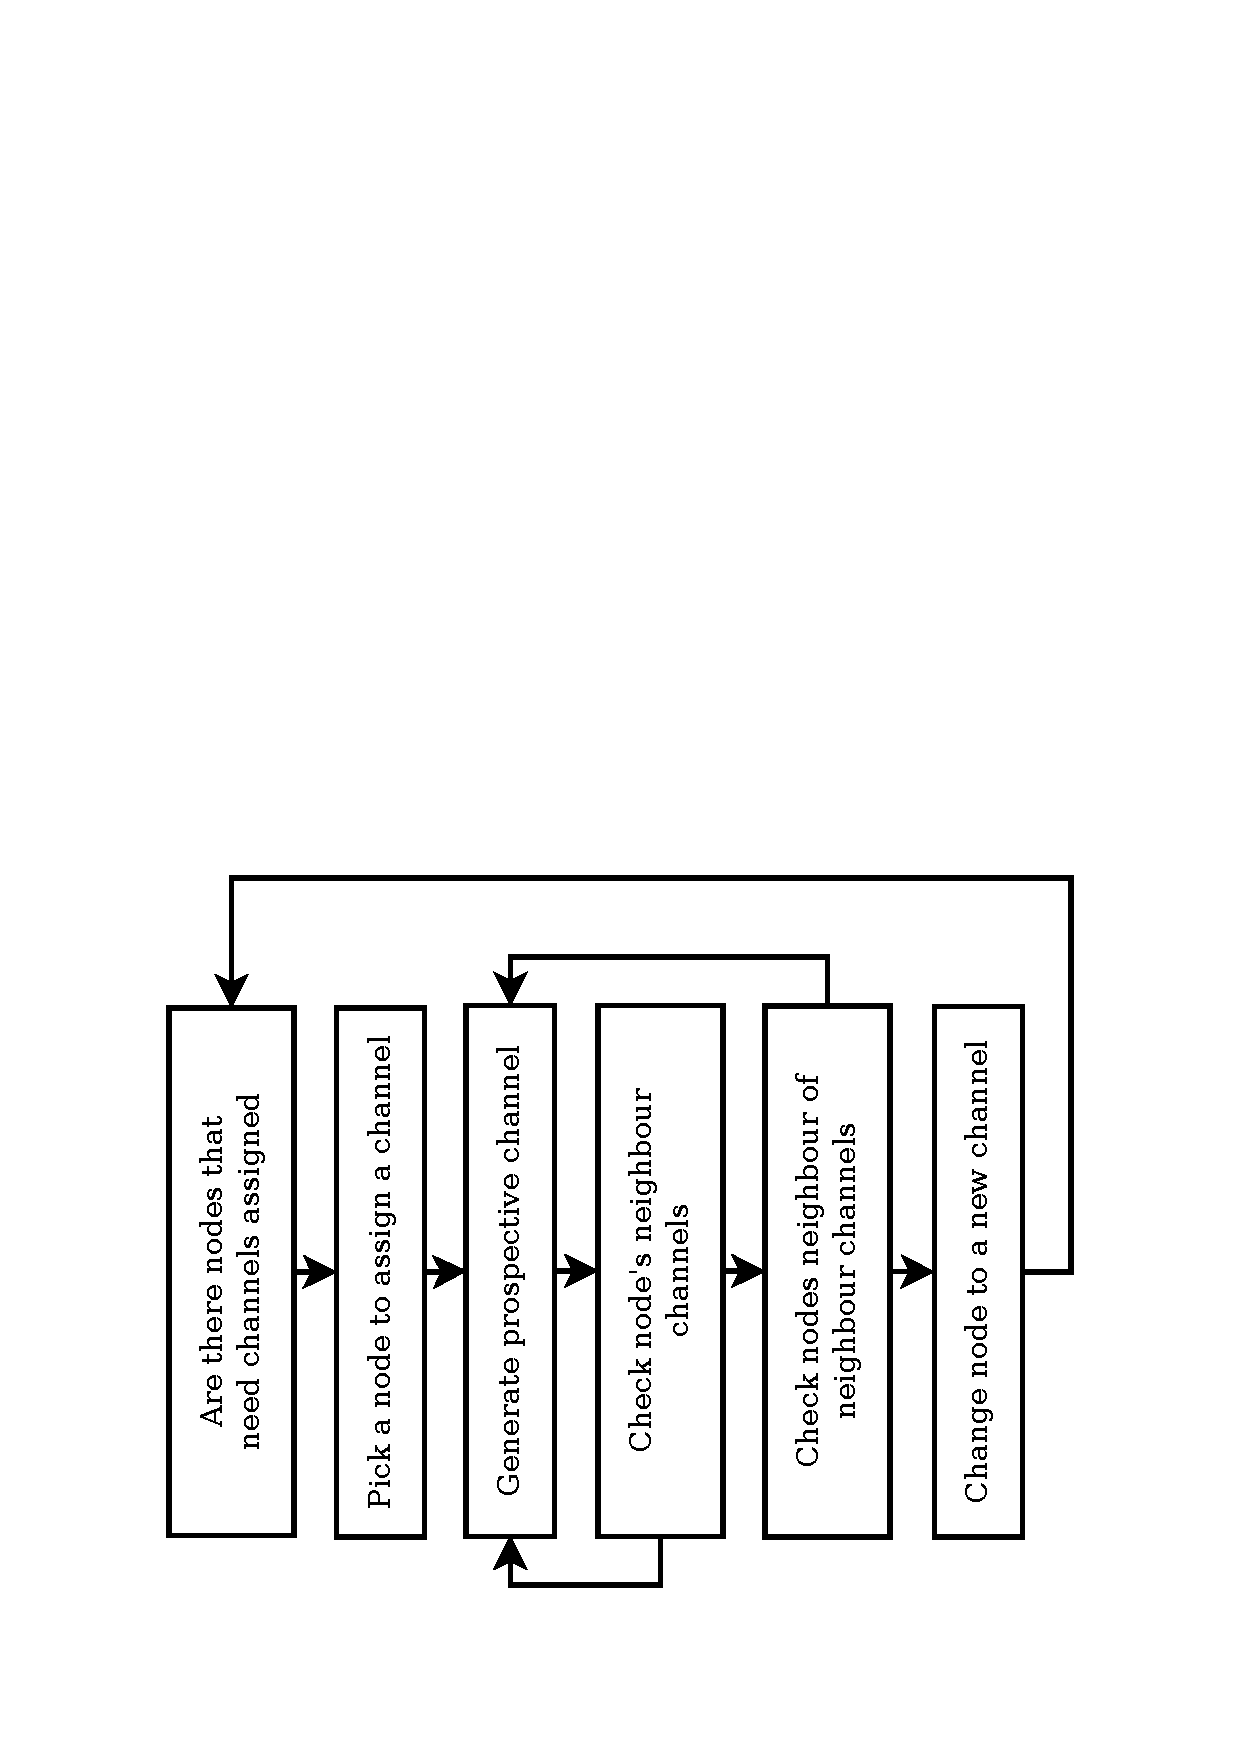
\includegraphics[trim=2cm 2cm 2cm 14cm, clip=true, totalheight=0.35\textheight, angle=270]{channelSelectionModified.pdf}
\caption{Channel selection strategy}
\label{fig_channelSelection}
\end{figure}
 
All nodes are initialised to channel 26 which is the common default channel for Contiki MAC layer since it often has fewer interference problems with Wi-Fi and other sources. The studies in \cite{chrysso, micmac, watteyne} use a set list of whitelisted channels in their experiments and have channel 26 in common. The usual RPL set up mechanism is used to exchange control messages that are required to form an optimised topology before channel assignments can take place. The nodes will only be on the same channel once during the initial setup.
This enables the node to detect and find nearby neighbours that are in range before it can decides on the best route based on the list of neighbours it can be connected to. 

In the two-hop colouring algorithm, the LPBR chooses a node to which it will assign a channel to listen on. The selection is random (from channels 11 to 26) based on the full range available \cite{ieee802.15.4}. The channels that were tested to have severe interference for one node might gives good result for another node depending on the location of the node which might not be within the range of where the channel has severe interference previously. MCRP has its channel quality checking mechanism before it decides on a channel which allows random channel selection to take place.

%The value is random - no need to pseudo-random number generators to avoid node persistently generating the same numbers as the channel that is bad for one node might gives good result for another node depending on the location of the node which might not be within where the channel is bad at. 

The protocol checks neighbours and neighbours of neighbours to see if any of those are listening on this channel already. If any are, a new channel is picked from the remaining list of available channels. If the LPBR has knowledge of existing bad channels then those channels can be blacklisted.  Knowledge of channel interference which is gained by probing can be used to decide that a channel should not be used. If a channel is found then the channel switching protocol is triggered. If no channel can be found meeting these conditions, the current channel is kept. Figure \ref{fig_channelSelection} summarised the strategy in LPBR channel selection. 

The node selection algorithm must only attempt one channel change at a time to ensure probing is done on the correct new channel and for the node to finalise the channel to be used before another node attempts a channel change.
The protocol ascertains that the channel change attempt will always result in a message returned to the LPBR either confirming the new channel or announcing a reversion to the old channel. Until one or other of these happens, no new channel change will be made to enable the neighbours transmitting on the correct channel.

\section{Channel Switching}

\begin{figure}
\centering
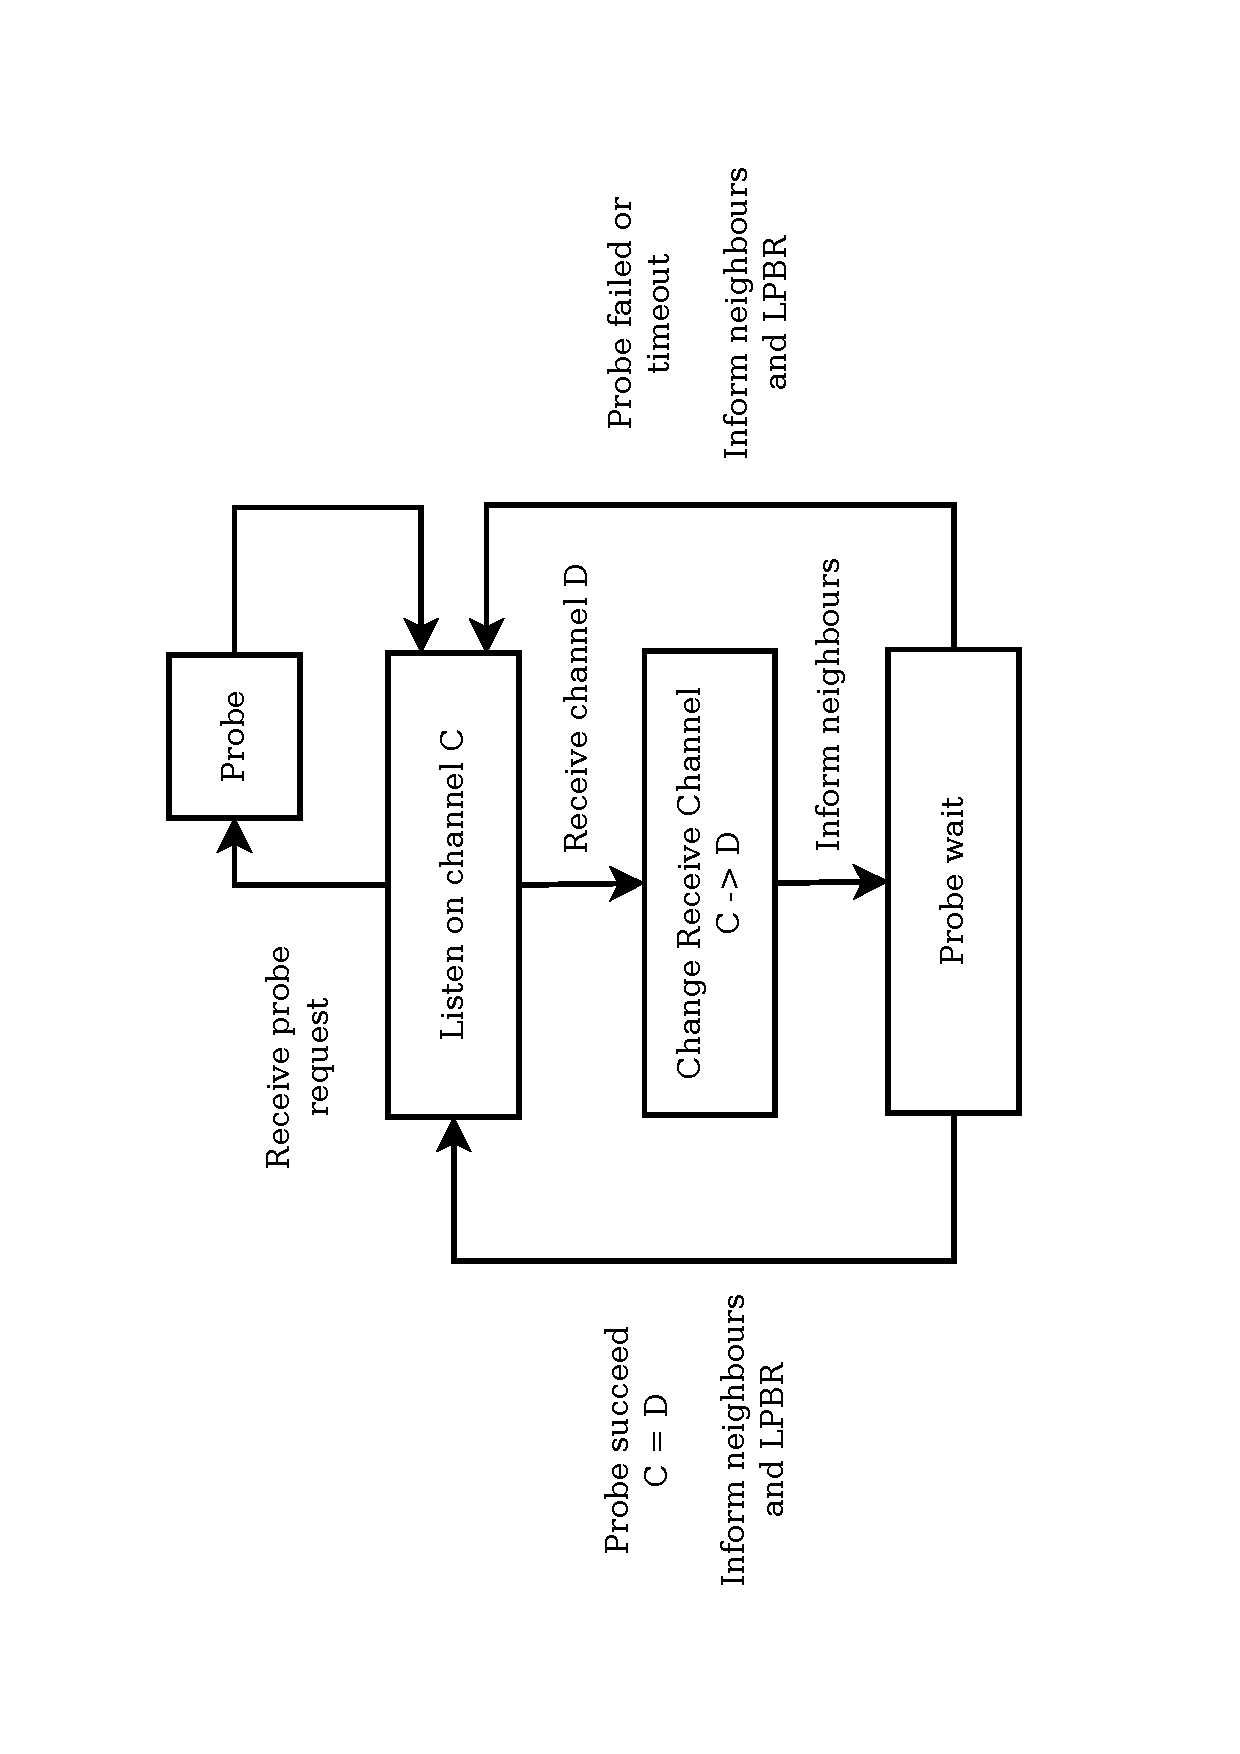
\includegraphics[trim=2cm 2cm 3cm 2cm, clip=true, totalheight=0.6\textheight, angle=270]{channelSwitching.pdf}
\caption{Channel switching processes}
\label{fig_mcrp}
\end{figure}

Figure \ref{fig_mcrp} shows the state machine for the channel switching protocol.
As explained in the previous section, a choice of a new channel by the channel selection protocol causes a change channel message to be sent to the appropriate node. 
Upon receiving a channel change message, a node $N$ stores its current channel $C$ and communicates to all its neighbours the new channel $D$ that it wishes to change to. Those neighbours will update their neighbour tables to ensure that they now send to node $N$ on channel $D$.  The node $N$ begins the channel quality checking process with each neighbour in turn by sending them a probe request. If this process fails for any neighbour then the node reverts to channel $C$. If all channel quality checks succeed, the node $N$ will listens on channel $D$. In both cases, node $N$ informs its neighbours of the decision to channel $C$ or $D$ and informs the LPBR of the channel checking results. The channel checking process uses probe packets that might interfere with other transmissions temporarily. However, it is important to emphasise that the network remains fully functional and connected at all stages of this protocol.

\section{Channel Quality Checking}
The channel quality checking is invoked each time a node changes channel after receiving a message from the LPBR. A node $N$ changing to channel $D$ informs all neighbours in turn, of the new channel $D$ it will be listening on as described in the previous section. It then enters the \emph{Probe Wait} state and begins channel quality checking with each tree neighbour in turn. In describing the channel quality checking process, it is worth emphasising the distinction between neighbours and tree neighbours. Node neighbours are all nodes that a given node knows it could transmit to. Tree neighbours are the nodes that a node does transmit to through the topology formed by the RPL protocol. 

In the \emph{Probe Wait} state, node $N$ sends a \emph{Probe} message to each neighbour in turn. The neighbours respond to the message by sending eight packets to $N$ on the new channel $D$. 
The buffer can accommodate eight packets at a time. As the packets might not be sent immediately due to wakes up and collisions, sending more packets would have the risk of being dropped. 
The condition of the channel is further investigated through the number of retransmissions and packet collisions of the probing packets for accuracy of the channel condition. 

If the probing process times out (because of some communication failure) or the number of probe packets received is above a threshold (currently set to 16, including retransmissions and collisions) then node $N$ immediately exits \emph{Probe Wait} state and reverts to channel $C$ its previous channel. 

All neighbours are informed of the change back to channel $C$ and the LPBR is informed of the quality check failure with a summary of all probes received.
If, on the other hand, all channel quality checks succeed, the change to channel $D$ becomes permanent for node $N$ and it informs the LPBR of the results of the probing (numbers of packets received) and the channel change.

Probing is essential to make the channel change decision. It gives a quick overview of the channel condition based on the number of probing messages received. It is worth noting that probing is only done between the node and the tree neighbours. Neighbours that are not tree neighbours will not use the node as a route during their transmission thus, there is no need for probing to take place with those neighbours. However, the neighbours still need to know the channel value given that RPL control messages are sent to neighbours directly without using the routes.

\section{Reconnection Strategy}
RPL topology stability (using routing metric) remains the same in multichannel \cite{routingmetrics, winter2012rpl}.
%RPL topology could change according to the routing metric \cite{routingmetrics} the way the usual RPL would work \cite{winter2012rpl}. 
The nodes can still change the parents as usual as all neighbours know each other new channels. The neighbours that are not part of the route do not probe the parent when making the channel decision. However, the neighbours are informed of any channel changes.

This enables the topology to be optimised when communication fails and further improved through MCRP as the nodes have knowledge of the listening channels of all other nodes within the range. If a new node tries to join the topology, it sends a RPL control message through all channels as the listening nodes are unlikely to be on the default channel. 

The listening nodes send a broadcast on a default channel to discover new nodes (in Contiki default, new nodes will start on channel 26) and send RPL messages through unicast when the neighbours are known to reduce unnecessary transmissions in broadcast. New nodes and nodes which fall off the network can now rejoin on many potential channels. %(20-25 pages)
\chapter{Implementation}
\label{implementation}

MCRP is implemented on the TelosB mote platform. It uses Contiki, a lightweight operating system as the software development platform that supports the standard IPv6. The implementations of MCRP across the layers in Contiki are described in details, specifying the changes that were introduced and undertaken in addition to the default parameters and settings in Contiki.

%Contiki is a lightweight operating system with support for dynamic loading and replacement of individual programs and services. The purpose of the Contiki design is to reduce size and complexity, as well as to preserve flexibility. A running Contiki system consists of the kernel, libraries, the program loader and a set of processes (may be either an application program or a service - functionality used by more than one application process e.g. includes communication protocol stacks, sensor device drivers) \cite{contiki}. 
 
%\section{Contiki Protocol Stack (changes at MAC, RT, NBR TB, BR etc.)}
\section{Contiki}
%MCRP is a cross layer protocol implemented on Contiki version 2.7. (explain what is cross layer? why do cross layer? FIGURE OF STACKS)

\begin{table}
  \centering
    \begin{tabular}{|c|c|c|}
      \hline
      Contiki & IoT/IP & Applications \\
      \hline \hline
      \multirow{4}{*}{Network} 
        & Application & HTTP \\
        \cline{2-3}
        & Transport & TCP, UDP \\
        \cline{2-3}
        & Network, Routing & IPv6, IPv4, RPL \\
        \cline{2-3}
        & Adaptation & 6LoWPAN \\
      \hline \hline
      
      MAC & MAC & CSMA/CA \\
      \hline
      RDC & Duty Cycling & ContikiMAC \\
      \hline
      Radio & Radio & IEEE 802.15.4 \\
      \hline
    \end{tabular}
    \caption{Contiki network stack}
    \label{table:1}
\end{table}

Contiki is defined by four layers network stack: the network layer, the MAC layer, the radio duty cycling (RDC) layer and the radio layers. The network layer includes support for TCP, UDP, IPv6, IPv4, RPL routing protocol and 6LoWPAN. IPv6 over Low Power Wireless Personal Area Networks (6LoWPAN) is a header compression and fragmentation format for IPv6 packets delivery over IEEE 802.15.4 networks \cite{6lowpan}. Contiki implements the minimal set of IPv6 protocol required, 6LoWPAN adaptation layer for IPv6 header compression and fragmentation which is routed over the low power and lossy networks (LLN) in RPL.

Contiki's configuration options for communications, buffer management and network interface are explained before looking into MCRP implementation for ease of reading.

%6LoWPAN working group specified header compression and fragmentation for IPv6 over IEEE 802.15.4 (///REFERENCE!!!) and the IETF RoLL working group designed the RPL protocol as a proposed standard for IPv6 routing in low-power and lossy networks (LLNs). Contiki implement the necessary parts of the IPv6 protocol, IPv6 header compression and fragmentation with the 6LoWPAN adaptation layer, routing over LLNs with the RPL protocol, as well as a set of protocols from the TCP/IP protocol suite \cite{beyondInteroperability}.

%///RPL does not rely on any particular features of a specific link-layer technology.  RPL is designed to be able to operate over a variety of different link layers, including ones that are constrained, potentially lossy, or typically utilized in conjunction with highly constrained host or router devices, such as but not limited to, low-power wireless or PLC (Power Line Communication) technologies.\cite{winter2012rpl}

\subsection{Communication Stacks}
\label{commstack}
Contiki contains two communication stacks, uIP and Rime.
uIP \cite{uip} is a small RFC-compliant TCP/IP stack that is designed to contain only the essential (required/necessary) features to provide Contiki with TCP/IP networking support to allow Contiki to communicate over the Internet compared to the traditional TCP/IP that requires (high) resources to fit in a limited RAM capabilities of a sensor. The minimal set of features includes IP, ICMP, UDP and TCP protocols compared to the traditional TCP/IP that requires (high) resources that could not be supported in the limited RAM capabilities sensor. The uIP is mostly concerned with the TCP and IP protocols and upper layer protocols \cite{contikiDoc, contikiUIP}. 

Rime is Contiki's lightweight communication stacks that aims to simplify the sensor network protocols implementation by reusing code in a layered manner \cite{rimeposter}. Rime combines layers of simple communication abstractions to form a powerful high-level abstraction ranging from best-effort anonymous broadcast to reliable network flooding. Parts of the Rime stack can be used by the underlying MAC or link layer. Additional protocols that are not in Rime can be implemented on top of the stack.

Applications in Contiki can decide to use one of the communication stacks available, both or none at all. uIP can run over Rime and similarly, Rime can run over uIP \cite{contikitutorial}. 

%Rime communication stack provides a set of lightweight communication primitives ranging from best-effort anonymous local area broadcast to reliable network flooding. Protocols or applications running on top of Rime stack can implement additional protocols that are not in the Rime stack such as TCP/IP.

%Rime draws heavily from communication abstractions for distributed programming.

%draws heavily from communication abstractions for distributed programming where layers of simple abstractions are combined to form powerful high-level abstraction. The purpose of Rime is to simplify implementation of sensor network protocols and facilitate code reuse. The thin layers in Rime enable code reuse within the stack. An underlying MAC or link layer may chose to implement parts of the Rime stack \cite{rimeposter}. 

%Traditional TCP/IP implementations have required far too much resources which is impossible to fit in a sensor that has limited RAM capabilities (RAM is the most scarce resource). uIP \cite{uip} is a small RFC-compliant TCP/IP stack that makes it possible for Contiki to communicate over the Internet. uIP implementation is designed to have only the absolute minimal set of features needed for a full TCP/IP stack such as IP, ICMP, UDP and TCP protocols. The uIP is mostly concerned with the TCP and IP protocols and upper layer protocols \cite{contikiDoc, contikiUIP}. 

\subsection{Buffer Management}
\label{bufmgmt}
Chameleon \cite{rime} is a communication architecture in Contiki that consists of Rime communication stack and a set of packet transformation modules. It uses an abstract representation of the information which allows access to the low-level features of the underlying MAC and link layer protocol from the applications and layers implemented on top of the Chameleon architecture. It also allows the output from the protocol stack to be adapted by other communication protocols. In Chameleon architecture, the parsing of its header is separated from the communication stack. This allows uIP or Rime communication stack to be used as described in Section \ref{commstack}. Chameleon architecture enables the layers to access information without violating the layering principle. 

%other communication protocols such as link and MAC layer protocols and TCP/IP. -input output?

%It allows access to the features of underlying MAC and link layer protocols for the implemented protocols on top of the architecture. 

%The use of packet attributes makes it possible to adapt the output from the protocol stack to other communication protocols such as link and MAC layer protocols and TCP/IP.

%Chameleon is a header construction. The parsing is done separately from the communication stack which allows the use of uIP or Rime communication stack that both are supported in Contiki.

%\cite{rime} introduces Chameleon, a communication architecture for sensor networks consists of Rime communication stack and a set of packet transformation modules. Rime communication stack provides a set of lightweight communication primitives ranging from best-effort anonymous local area broadcast to reliable network flooding. Protocols or applications running on top of Rime stack can implement additional protocols that are not in the Rime stack such as TCP/IP.

%Chameleon does not define any packet headers but instead uses $packet attributes$, an abstract representation of the information usually found in packet headers to allow applications to access low-level information without violating the layering principle. Packet headers are produced by separate header transformation modules that transform application data and packet attributes into packets with header and payload. The use of packet attributes makes it possible to adapt the output from the protocol stack to other communication protocols such as link and MAC layer protocols and TCP/IP.
%Chameleon architecture allows for sensor network protocols that are implemented on top of the architecture to take advantage of the features of underlying MAC and link layer protocols.

In buffer management module of Chameleon architecture, all incoming and outgoing packets from the applications and packet attributes are stored in a single buffer called the Rime buffer \cite{uip, rime, rimeposter, contiki}. All layers of Contiki's network stack including uIP, Rime and the underlying link layer operate on the same packet buffer for the buffer management. The Rime buffer has no locking mechanisms as it is a single priority level buffer. The buffer only holds the current packet.

Protocols that need to queue packets allocate the queue buffer dynamically. Queue buffer is used to hold the queued packets such as for MAC protocols that have high rate of incoming and outgoing messages before it can send or process the receiving packets; or when the radio is busy and the MAC protocol has to wait for the radio medium to be free before proceeding with transmissions. Queue buffer is used to avoid the risk of the packet overwritten by the newer packet. The Rime buffer contents are copied into the queue buffer when there is a queue buffer allocated.

%Protocols that need to queue packets, such as MAC protocols that wait for the radio medium to be free, can allocate so-called queue buffers to hold the queued packet. Queue buffers are dynamically allocated from a pool of queue buffers. The contents of the Rime buffer, including the packet attributes, are copied into the queue buffer when it is allocated.

%All layers of the netstack operate on the packet buffer. 
%Rime's buffer management module is used by the underlying link layer for buffer management.
%The packet buffer only holds the current packet.

%Even though it is called a Rime buffer, both uIP and Rime uses the same buffer.

%In the buffer management of Chameleon architecture, all packets both outgoing and incoming are stored in a single buffer \cite{rimeposter}, called the Rime buffer. 
%The Rime buffer contains both the application data and the packet attributes. All access to the Rime buffer is done at a single priority level so no locking mechanisms need to be used.

%Rime's buffer management module is used by the underlying link layer for buffer management.
%////BUFFER MANAGEMENT - since it's related to uIP (Chameleon, Rime etc)

%All layers of the netstack operate on the packet buffer. One buffer holds a single packet. ***Uses a single buffer for both incoming and outgoing packets \cite{uip, rime, rimeposter, contiki}. The packet buffer only holds the current packet.

%Buffer for uIP and Rime is the same. They use the same buffer.
%\subsection{Retransmission} 


%It uses (EXPLAIN CONTIKIMAC - refer to contikimac paper; why it's good, how it works). Also about retransmission and buffers. (maybe at next section???) The transmitting channel is set at the MAC layer as packets are not send immediately if there are packets being queued. The channel is reset to the transmitting channel before it tries to send and it is then reset to the listening channel to wait and listen to any packets that is being sent to the node. 

%The default ContikiMAC is a single channel protocol. It is modified to be able to work with multi channel nodes while (stick/hold/is) on the same principle of a low power ContikiMAC (minor changes to support multi channel without changing the main purpose of ContikiMAC).

\subsection{Tunslip}
Serial Line Internet Protocol (SLIP) \cite{slip} is a protocol that has a low complexity and small overhead commonly used to encapsulate IP packets for point-to-point communication between the sink (LPBR) and the device connected such as an embedded PC across the serial connections. The communication between the devices can take place on any reliable network such as the Ethernet where the LPBR can be connected to an embedded PC which contain an Ethernet interface.
%which the interface is available in the embedded PC.

%Serial Line Internet Protocol (SLIP) //need reference!!!] is used for the communication between the sink and the device which it connected to such as an embedded PC. 
%SLIP is commonly used to encapsulate IP packets for transmission across the serial line of micro-controller devices. 
%SLIP has a low complexity and small overhead. 
%For the communication between the devices (embedded PCs), any reliable network can be used (e.g. Ethernet). 
%The sinks are connected to an embedded PC which contains an Ethernet interface. The communication between the sink (sensor node) and the embedded PC makes use of SLIP. 

Contiki provides support to communicate with devices using SLIP through its tunslip tool. Tunslip is used to bridge the IP traffic between the LPBR and the embedded PC over a serial line. The other side of the serial line does a similar job to bridge the embedded PC to the LPBR using the network interface. It constructs a SLIP tunnel between a virtual network interface (tun) and SLIP, the physical serial interface to encapsulate and pass the IP traffic to and from the other side of the serial line. The tun interface is used as any real network interface such as for routing and traffic forwarding \cite{tunslip, multipleSinks}.

%Contiki already provides support for SLIP communication and includes a tunslip tool (need reference!!!) which make it possible to communicate with devices using SLIP. 
%The tool constructs a SLIP tunnel between a physical serial interface and a virtual network adaptor. 
%By using tunslip the communication between the sink and the embedded PC is facilitated \cite{multipleSinks}.

%Tunslip is a too used to bridge IP traffic between a host and another network element, typically a border router, over a serial line. 
%Tunslip creates a virtual network interface (tun) on the host side and uses SLIP (serial line internet protocol) to encapsulate and pass IP traffic to and from the other side of the serial line. 
%The network element sitting on the other side of the line does a similar job with it's network interface. 
%The tun interface can be used like any real network interface: routing, traffic forwarding etc \cite{tunslip}.


\section{MCRP Implementation}
MCRP is implemented in Contiki and uses ContikiMAC as the MAC protocol, RPL as the routing protocol. ContikiMAC is modified to allow multi channel where the channel selection processes take place on the upper layers and the channels are kept in the network neighbour table to ensure the correct channel.

The protocol implementation is separated into two types of nodes: i) the centralised LPBR where the bridging takes place between the border router on a PC to the nodes, and ii) the decentralised transmission nodes referred as other nodes. The implementation for both types are described below.

%MCRP is implemented as an extension to the existing implementation of RPL with ContikiMAC; to enable multi channel.
%The protocol is implemented by tailoring existing code of ContikiMAC, network layer and RPL.

%\subsection{Application Layer}
%//separate into 2; setCh and xSetCh as LPBR is separated with BR and SR
%//access Network layer - Neighbour table, set channel

\subsection{Low Power Border Router}

\begin{figure}
\centering
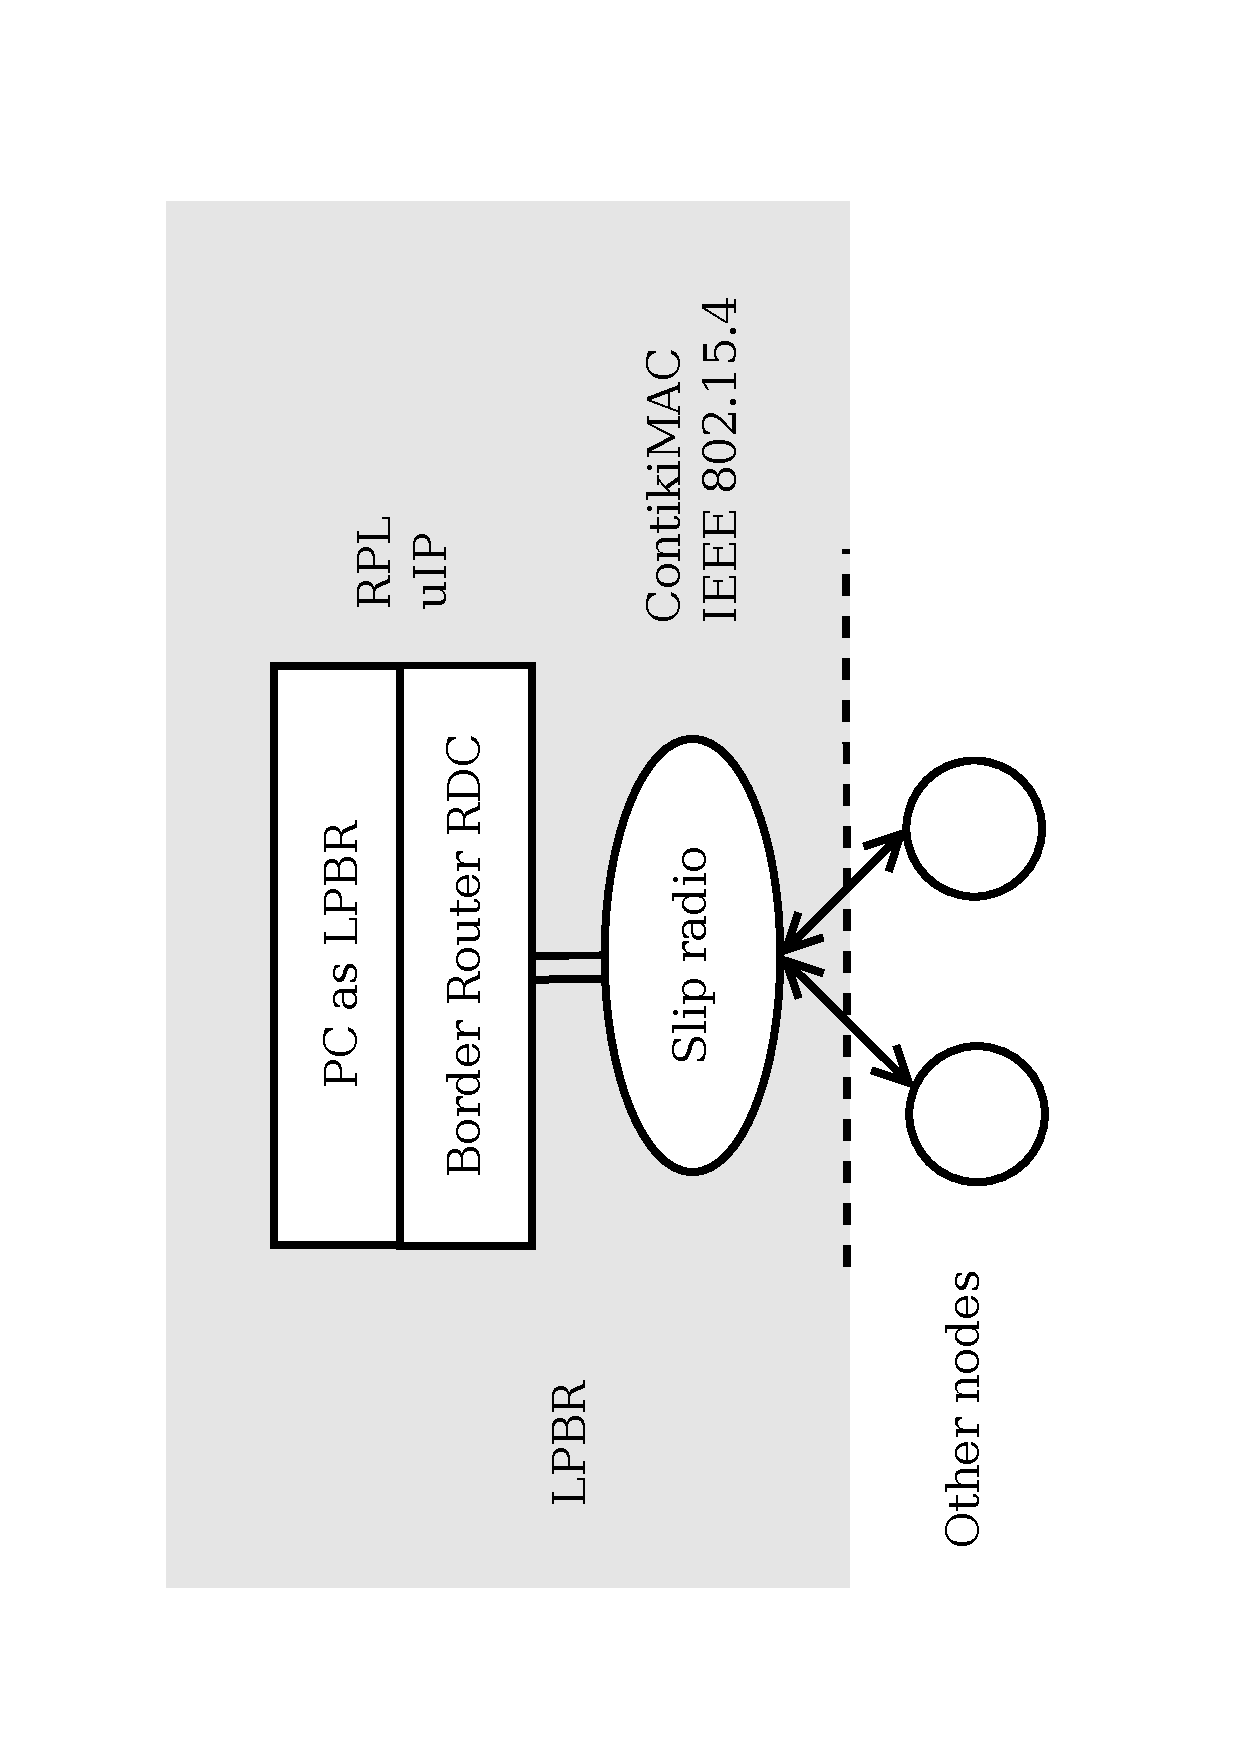
\includegraphics[trim=2cm 2cm 3cm 2cm, clip=true, totalheight=0.45\textheight, angle=270]{BR2.pdf}
\caption{Low power border router}
\label{fig_lpbr}
\end{figure}

As sensors have limited memory, most processing decisions at LPBR are transferred to a PC as it has more RAM and better processing capabilities. This enables MCRP to have more thorough processes and to run in real time without draining the memory and battery on a sensor. LPBR is divided into two main parts as shown in Figure \ref{fig_lpbr} where the PC is responsible as the application, transport, network and routing layers while a sensor (labelled slip radio) is set as the wireless interface to enable the PC to communicate with the other nodes via Contiki tunslip tool. 

The LPBR acts as the tree root in RPL where it will initiate the creation of the RPL routing tree. LPBR is a special case as channel changes at LPBR is not as direct as other sensor nodes due to this two parts. However, it works similar ways to the other nodes.

%It (tunslip6) sets up an interface on the Linux IP stack and connects this interface via a socket to the border router node.
%Border router is used to bridge the wireless IPv6 network to a PC via serial link which enables the IPv6 network traffic to reach outside network and the Internet.
%A node is used as a wireless interface (IEEE 802.15.4 to enable the serial socket server), a host machine as border router to bridge the wireless IPv6 network to outside network and the Internet.

%trim top left

LPBR main responsibility is to decide on the new channel selection. LPBR has no knowledge of all the channels condition at this point, thus, a channel is selected at random. LPBR keeps the results from the channel changes processes and based on it when selecting a new channel for the next node to ensure the new channel is at least two-hop away from another node using the same channel. This is done to ensure that the nearby nodes do not communicate of the same channel and risk interfering with each other.

\begin{algorithm}
\caption{Pseudo-code for two-hop colouring algorithm}
\label{twohop_algo}
\begin{algorithmic}[]
\\\textbf{Notations}
\\$R$ is a node that is a Route
\\$N$ is a node Neighbour
\\$RN$ is the Route's Neighbour node
\\$currentCh$ is the node current listening channel
\\$newCh$ is the new channel the node will change to
%\\$rnCh$ is the route's neighbour channel
\\\textbf{Pseudo-code}
%\If{$R$ $=$ $R$ in $LPBR$ $nodesTable$}
%	\State check $R$ $currentCh$
	\If{$R$ $currentCh$ $\neq$ $newCh$}
		\State succeed one-hop
		\State check all $RN$ channels
		\If{$RN$ channel $\neq$ $newCh$}
			\State succeed two-hop
			\State confirm $newCh$
		\EndIf
	\Else
		\State generate a new $newCh$
		\State update the number of $newCh$ generated for $R$
		\State use default channel 26 is all tries fail
	\EndIf
%\EndIf
\end{algorithmic}
\end{algorithm}

The pseudo-code of the implemented two-hops colouring algorithm for new channel selection is shown in Algorithm \ref{twohop_algo}. When the new channel is selected, LPBR will send the value to the intended node.

%/////RPL border router is used as LPBR in order to move most processing decisions on a PC as it has more RAM and better processing capabilities than a sensor. (Explain BR-SR how it works!)
%TelosB has limited RAM and ROM of 10K bytes and 48K bytes of flash memory \cite{telosb-datasheet}. By using a border router, this allows channel changing to be decided in real time without draining the memory and battery on a sensor. The border router also acts as the root of the tree. The border router will setup the IPv6 prefix of the network and will initiate the creation of the RPL routing tree.
%It (tunslip6) sets up an interface on the Linux IP stack and connects this interface via a socket to the border router node.
%Border router is used to bridge the wireless IPv6 network to a PC via serial link which enables the IPv6 network traffic to reach outside network and the Internet.
%A node is used as a wireless interface (IEEE 802.15.4 to enable the serial socket server), a host machine as border router to bridge the wireless IPv6 network to outside network and the Internet./////

\begin{figure}
\centering
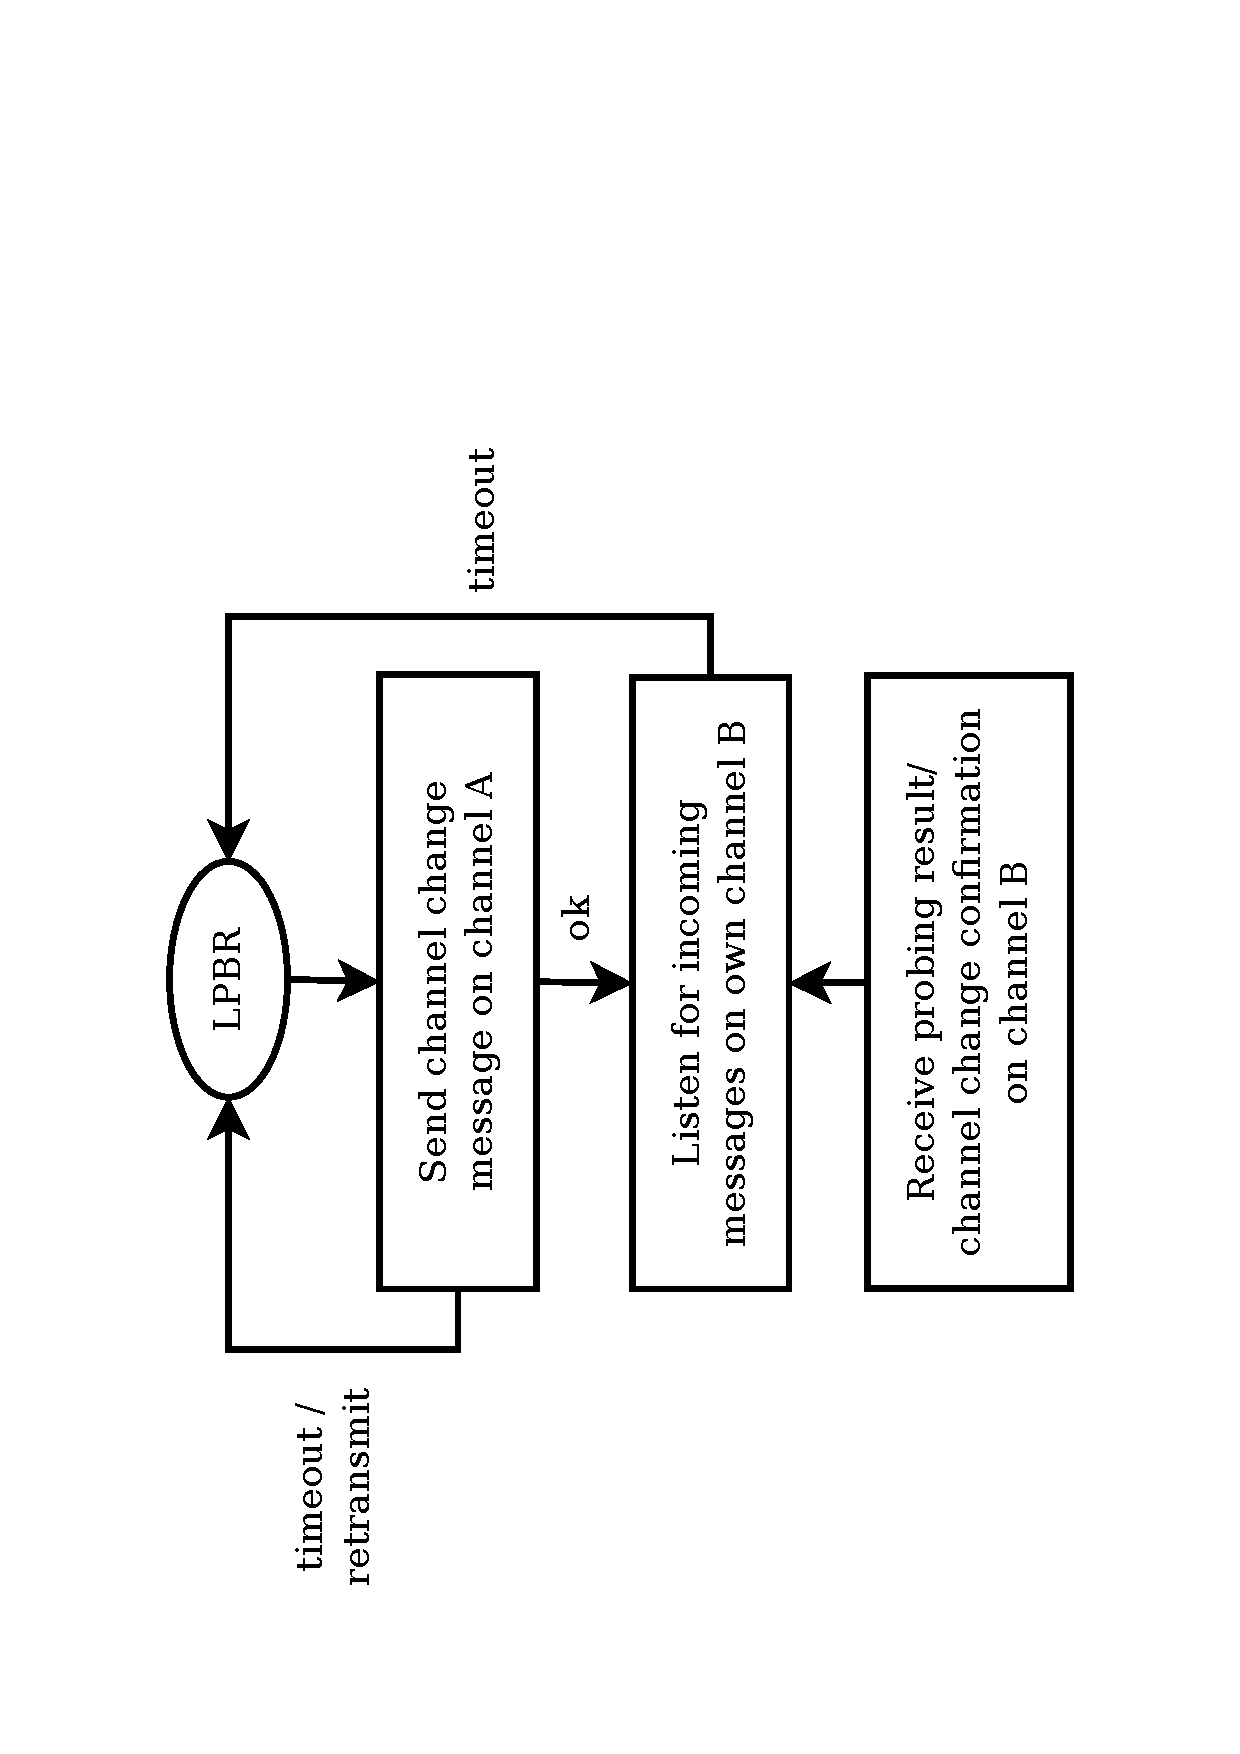
\includegraphics[trim=2cm 1cm 2cm 4cm, clip=true, totalheight=0.55\textheight, angle=270]{lpbrProcess.pdf}
\caption{LPBR processes}
\label{lpbrProcess}
\end{figure}
%top, left, bottom, right

The new channel is stored in the buffer before the data is sent over SLIP to the radio-chip (slip-radio). As the slip radio is unable to access the neighbour table where the next hop node channel is stored, the channel value is passed through the buffer. LPBR keeps the updated value of all it's neighbours channels in the neighbour channel. Slip radio that receives the packet buffer can access the channel value and kept the value is a simplified version of the neighbour table. This is done in order to ensure that the packet that is being queued or retransmitted are send on the correct channel. The packets destination, which in this case, the next hop node is first check before the packet is transmitted each time. The MAC layer sets the channel accordingly before sending. ContikiMAC can access the simplified neighbour table as it is on the slip radio. The simplified neighbour table only keeps the information of the node neighbours and neighbours channels which are the critical information in order to transmit packets correctly. The other information that is related to the neighbours conditions are monitored at the PC. 

LPBR processes are shown in Figure \ref{lpbrProcess}.
The slip-radio resets to it's listening channel after the packet is transmitted. LPBR will wait and listen to any incoming packets. In the channel probing phase, LPBR does not take part in probing. However, LPBR is informed of the results of probing and kept a table of the probing results and channels to be able to use the information when deciding on a channel change based on the previous results of probing on the known channels.

%Before passing to slip-radio, the header from $uip\_buf$ is compress to $packetbuf$. From $packetbuf$ to $uip\_buf$ is it decompress to access the data from the upper layers.  

%-send to BR RDC, check nbr table for the currentCh. pass the value to s-r. save the chvalue in a simplified nbr table to allow retx/queue to send on correct ch.
%MAC set the channel accordingly before sending.
%Change to its listening channel after finish sending. 

\subsection{Other Nodes}

\begin{figure}
\centering
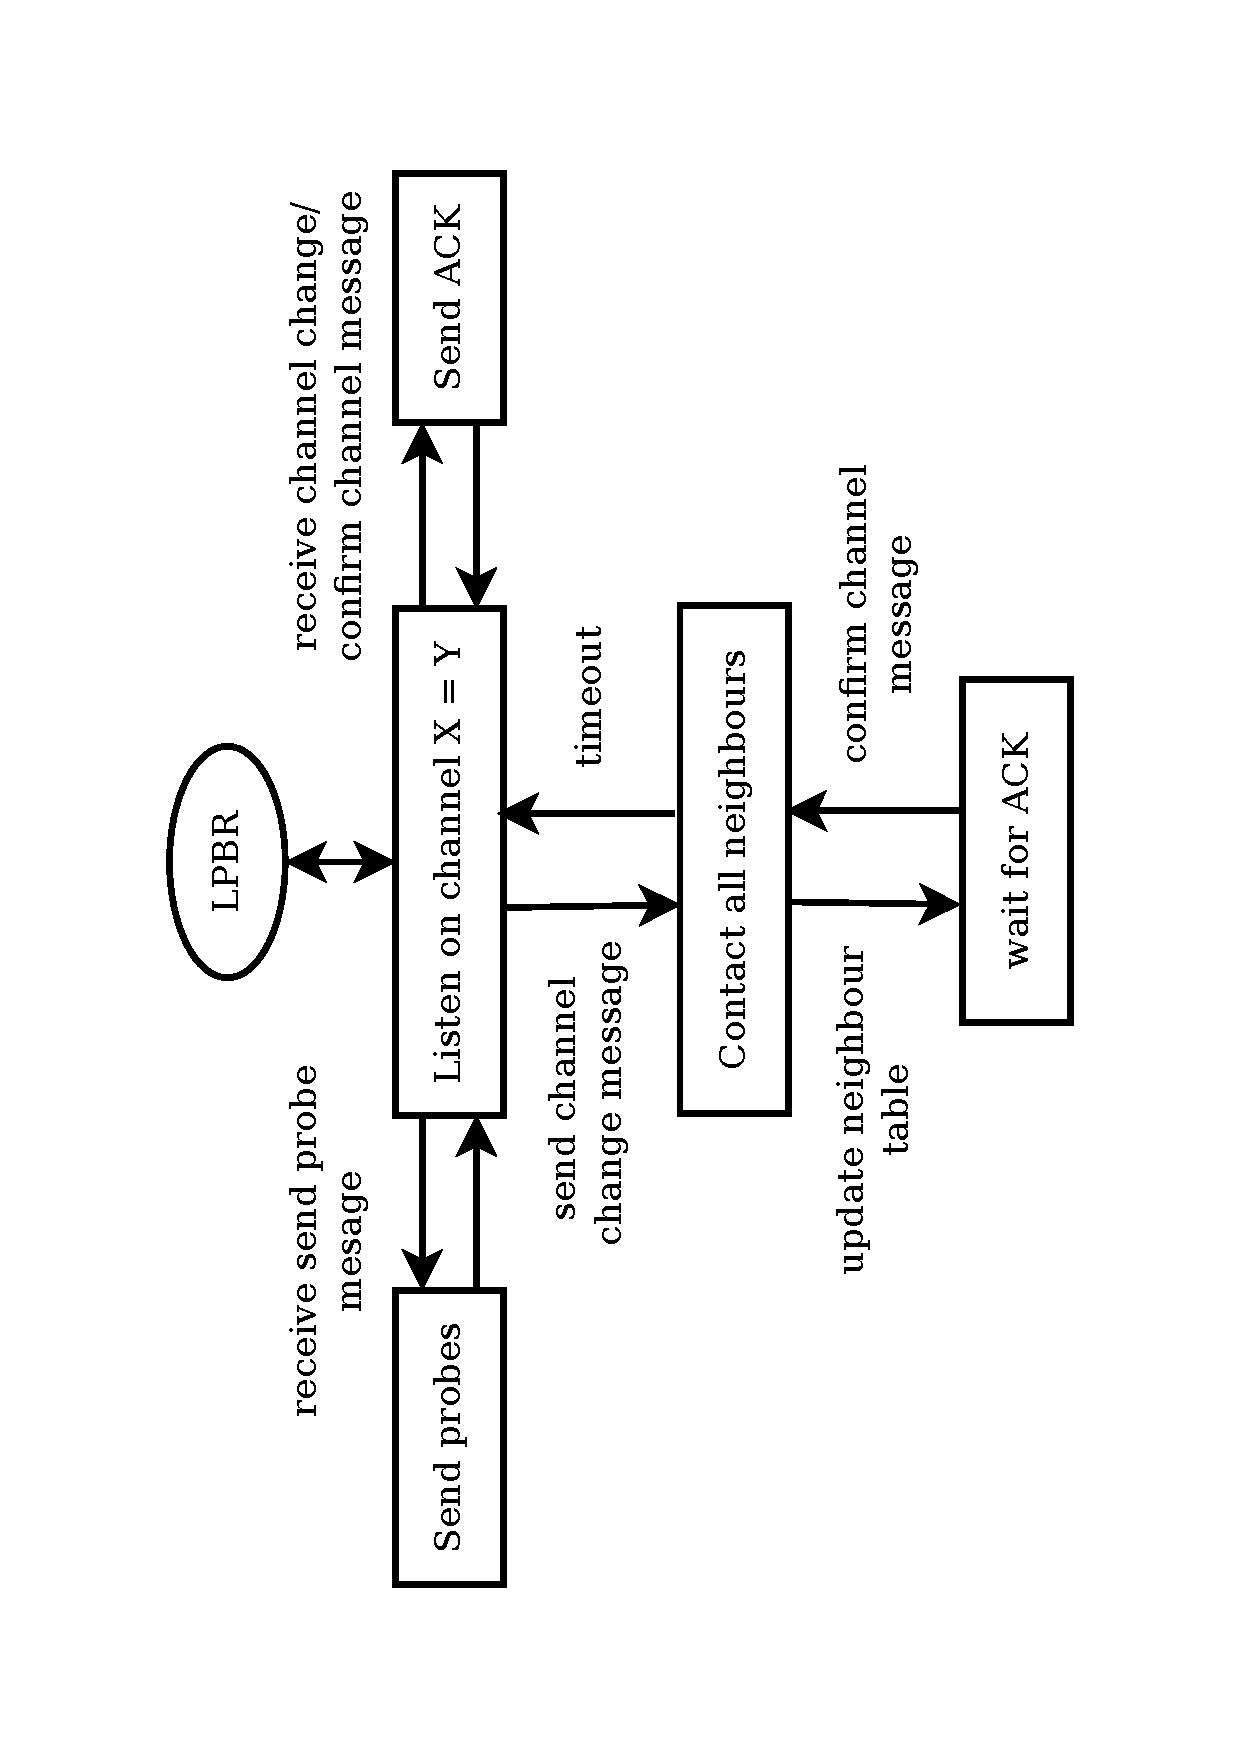
\includegraphics[trim=2cm 2cm 2.5cm 2cm, clip=true, totalheight=0.58\textheight, angle=270]{otherNodes.pdf}
\caption{Nodes channel change processes}
\label{fig_otherNodes}
\end{figure}

The new channel from LPBR that is received by the destination node is saved. 
Figure \ref{fig_otherNodes} shows the processes that the node takes in the channel change. When LPBR sends a \textit{Channel Change} message to the destination node, the destination node will send a packet back to LPBR to acknowledge the channel change message. If LPBR does not receive the message, the channel change message is retransmitted. LPBR will then wait and listens for any incoming packets. At this point, channel changes processes will take place between the node and its neighbours. To clarify, \textit{node} refers to the node that would like to change its listening channel and \textit{neighbour node} is the neighbour of the node (including route node) that takes part in the channel change decision through probe message.

%All nodes keep the neighbours channel in the \textit{neighbour table}. An entry is added in the neighbour table to hold the channel value called \textit{nbrCh}. 
Unlike LPBR, other nodes have all the layers within the nodes themselves. This makes channel changes less complicated, however, the nodes are being limited by the number of RAM they have which resulted in probing values to be stored in the centralised LPBR. The nodes however, keep the probing results temporarily before the final decision of the channel is made. 
%The nodes have cross-layer access. They can gain information from any layer when required.

The node sends the \textit{Node New Channel} value to all of the node's neighbours. At this point, the new channel is not yet checked for it's validity. However, all neighbours need to know the new channel as the node will change its listening channel to the new channel. Otherwise, packets cannot be received by the node since the listening channel is different than it was previously. The neighbours that receive the node's channel will update their \textit{neighbour table} which is accessed from the application layer. 
Unlike LPBR, other nodes have all the layers within the nodes themselves. This makes channel changes less complicated as the nodes can access the information from any layer when required which in this case, accessing the neighbour table at the network layer from the application layer.
In the neighbour table, a new entry is added to hold the channel value called \textit{nbrCh}. As this is an important step in order to reduce the number of packet loss due to sending on the wrong channel, neighbours will send an acknowledgement of the new channel. Otherwise, it will be retransmitted. 

The node will then send a \textit{Start Probe} message to the neighbour that is a route node to start sending probing messages on the new channel. Not all neighbours are used as routes. The neighbours are chosen as route based on RPL OF which for this experiment is the ETX. The node will listens on the new channel and wait for the \textit{Neighbour Probe} message. The route node starts to \textit{Send Probe} messages every 3 seconds to allow retransmission or collision that could happen due to the busy channel. The maximum number of retransmission is configured to 3 attempts following the default value Contiki suggested. Collisions happen when the channel check keeps failing and new packets are constantly generated which could end up in a loop where no packets can be sent. The assumption that was made in this case is the channel will be cleared at some point which this loop will not happen. From the experiments and simulations, this was proved true.

%(////what is retransmission? what is collision??? how it happens? how long? collision has no time out!). 
As only a small number of \textit{Send Probe} messages are sent, the number of retransmissions and collisions that happen during the probing process are included in the channel decision process as it affects the channel reliability.
%the we are sending a small number of probe message, to increase the channel reliability of the probing, we also take into account the number of retransmission and collision that happen. 
As the retransmission and collision is a link layer process, the values are kept in a temporary \textit{Retransmit Table} and is included to be sent in the next \textit{Send Probe} message. This is because the value is only valid for that run. It gets reset each time a new packet is sent or received. The table is accessed at the application layer before the next \textit{Send Probe} message is sent. The \textit{Send Probe} message includes the current number of probe message and the number of tries (retransmissions and collisions) the previous packet had taken before it is successfully received. These values are used to decide if the channel is better than the current channel by giving a good probing result, meaning less retransmission.

The node keeps the value of all probing messages it receives. It sends the \textit{Probe Result} message to LPBR. 
Unlike LPBR, the node has a limited RAM which resulted in past probing values to be stored in the centralised LPBR. The node however, keeps the probing results temporarily before the final decision of the channel is made. 
LPBR could use the information from the node's \textit{Probe Result} to decide on a channel or blacklist bad channels. 

The node then use the values to decide whether the new channel is better than the previous channel by setting a threshold. The node then send \textit{Confirm Channel} message to all neighbours that the node confirms to be listening on. The channel can be the new channel or the node can revert to the previous channel depending on the \textit{Probe Result}. The neighbours will send an acknowledgement back to the node confirming the change. This is also important to ensure that all neighbours could communicate with the node on the correct channel. The neighbours will update their neighbour table of the node channel. 

\subsection{MAC Protocol}
%As MCRP is a cross-layer protocol, 
As explained in Section \ref{bufmgmt}, packets that have not been transmitted are queued in the buffer. The transmitting channel is set at the MAC layer as packets are not send immediately if there are packets being queued. ContikiMAC is a single channel protocol. It is modified to support multi channel while complying to the same low power ContikiMAC principle. Each time the node goes to sleep, it will wakes up on its listening channel waiting for incoming packets. If the node has a packet to send, it needs to change to the transmitting channel.

In order for the packet transmission or retransmission to be on the correct channel, the neighbour channel saved in the \textit{neighbour table} at the network layer is accessed from the MAC layer and the channel is set to the transmitting channel. The node resets the channel to its listening channel after the transmission succeeded and goes back to sleep.

\begin{figure}
\centering
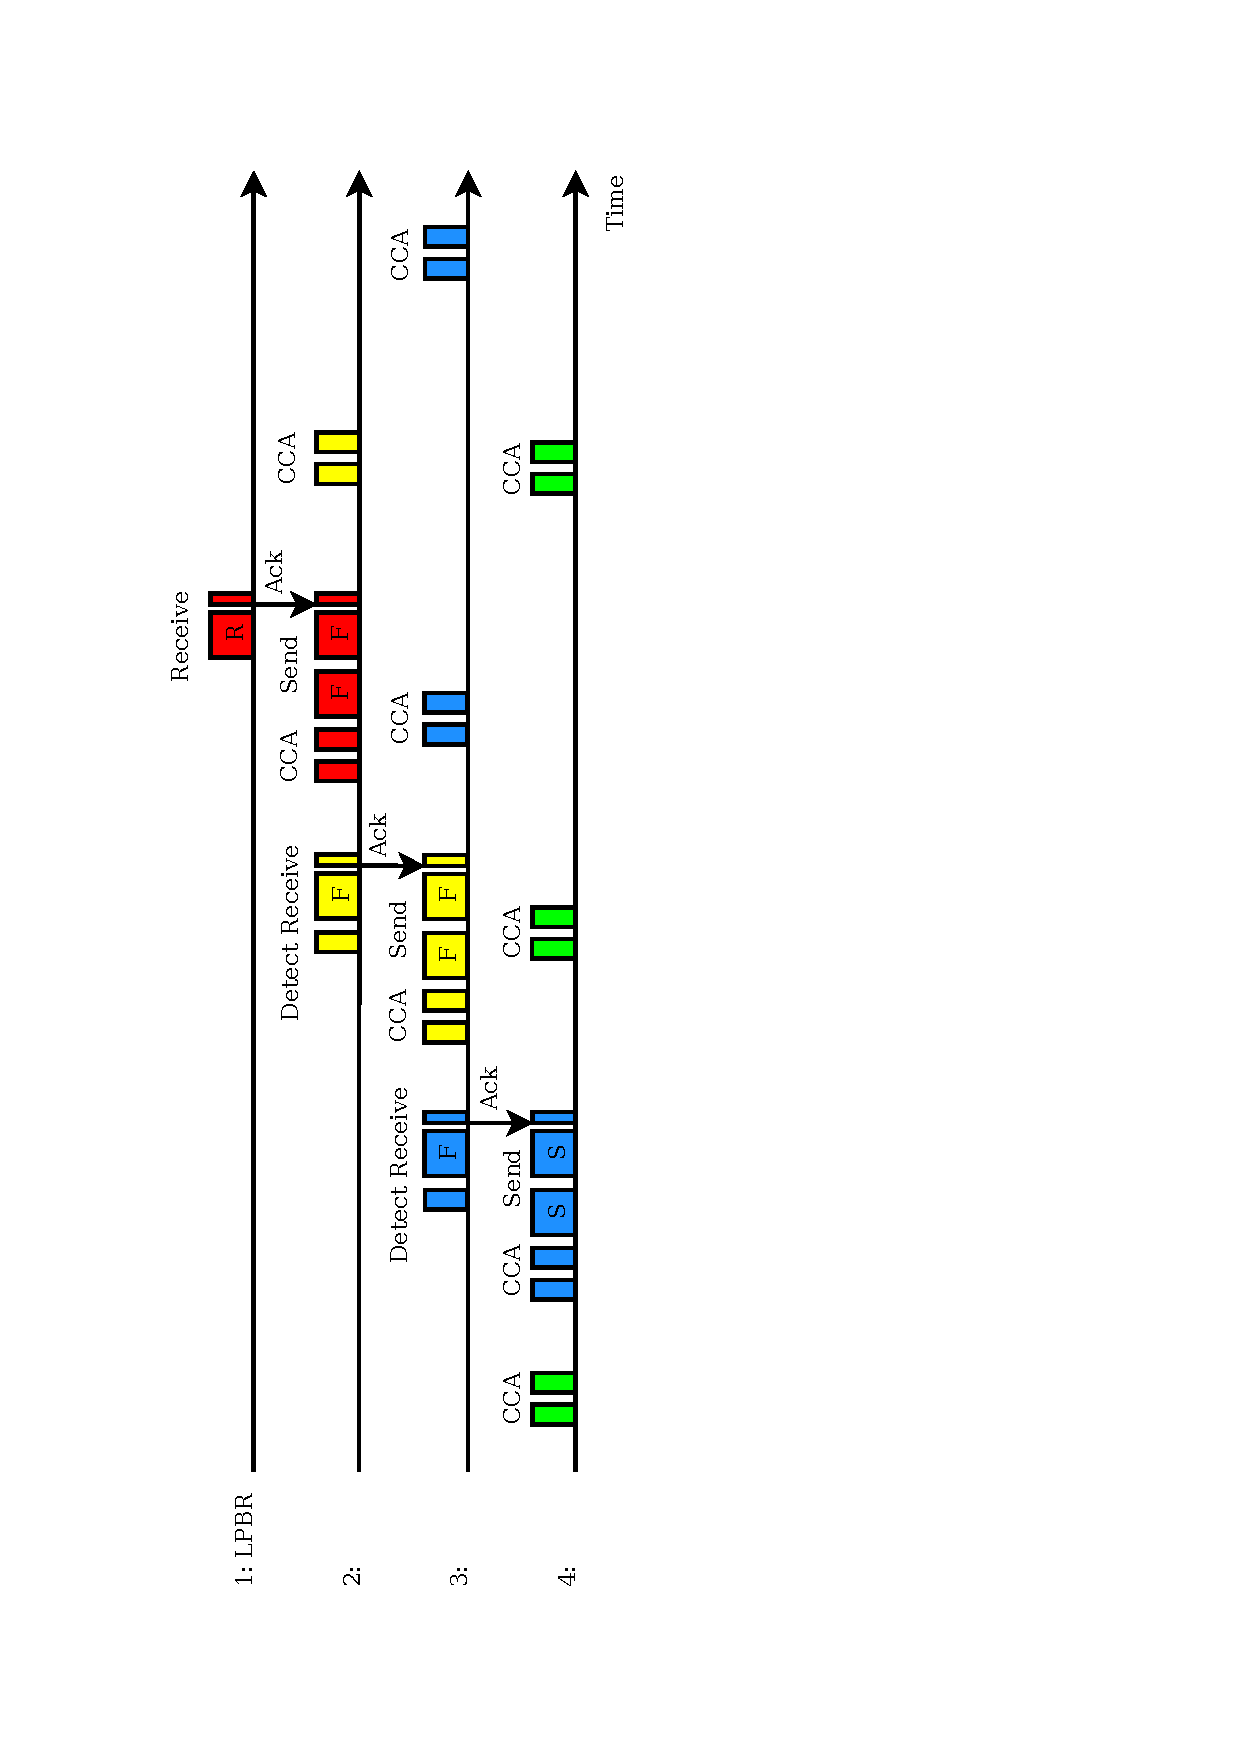
\includegraphics[trim=2cm 2cm 10cm 2cm, clip=true, totalheight=0.6\textheight, angle=270]{macExample2.pdf}
\caption{Multi channel ContikiMAC multi hop packet transmission}
\label{fig_mac}
\end{figure}

Figure \ref{fig_mac} shows an example of a multi hop packet transmission. At each hop, the node changes to the next hop listening channel before forwarding the packet. In the example, node 4 is sending a packet to node 1, the LPBR through node 3 and node 2. Node 4 wakes up and check for incoming packets on its channel. As it has a packet to be sent to node 1, it checks the next hop channel which is node 3 and changes the channel to node 3 listening channel. It checks if the channel is clear for transmission and proceed to send the packet to node 3. Node 3 detects the packet when it wakes up and receive the packet. Node 3 sends the link layer acknowledgement to node 4 so that node 4 stops sending the packet. Node 3 forwards the packet to node 2 on node 2 channel and node 2 to node 1, the LPBR which is the destination node. All nodes reset their channel after the transmission and wake up on their own listening channel. 

%If the node has a packet to send, it needs to access the neighbour channel to be able to transmit a packet on the correct channel. 

%ContikiMAC has retransmitted, collisions valued. These values are used in probing to decide on the channel condition. These values are passed to the application layer to decide on channel change. The packet can be retransmitted for ( ) times before it is dropped. However, if the channel is busy, and the packet has not been sent (collisions before sending), it can stay in the loop for a long time.

%//////It uses (EXPLAIN CONTIKIMAC - refer to contikimac paper; why it's good, how it works). Also about retransmission and buffers. (maybe at next section???) 
%The transmitting channel is set at the MAC layer as packets are not send immediately if there are packets being queued. 
%The channel is reset to the transmitting channel before it tries to send and it is then reset to the listening channel to wait and listen to any packets that is being sent to the node. 

%The default ContikiMAC is a single channel protocol. It is modified to be able to work with multi channel nodes while (stick/hold/is) on the same principle of a low power ContikiMAC (minor changes to support multi channel without changing the main purpose of ContikiMAC).//////

\subsection{Routing Layer - Neighbour Discovery}
///net/rpl/rpl-icmp6.c and rpl-timers.c - the changes done!!

RPL is explained in Section \ref{rpl}. RPL control messages are tailored to accommodate MCRP proposal by enabling unicast to know the neighbours and broadcast to detect new nodes to join the tree.

%RPL is used as the routing protocol. (explain how RPL works briefly since it's explained in LITERATURE REVIEW).

%We tailored RPL control messages to be able to accommodate MRCP proposal by enabling unicast to know neighbours and broadcast to detect new nodes to join the tree.  

////DIO UNICAST
RPL sends the control messages as broadcast. However, as we are now dealing with multi channels, using broadcast for all channels would waste the bandwidth and costly as it would take a longer time to go through all channels. It would also cause congestion and the node to be on the broadcast channel and not ready on it's listening channel to be able to receive any incoming packets as it has not finish with the control message broadcast. RPL DIO message is able to deal with either broadcast or unicast. By default, broadcast was used as RPL is usually used with a single channel MAC. We enable the unicast DIO.

////MULTI CHANNEL DIS
If a new node tries to join the tree, it will send a DIS message on all channels until it finds the neighbours. 

Two main changes that were done to RPL routing protocol is at the DIS (which is sent by a new node to make it possible for a node to require DIO messages from a reachable neighbor) and DIO (the main source of routing control information) control messages.

As we are dealing with multi-channel, a new node that would like to join an existing tree needs to send the DIS control message to the reachable neighbors. However, as the reachable neighbors could be on different channel than it were initially during start up, the new node needs to send the DIS message on all channels available. 

The neighbors that receive the DIS message will reply with a DIO message and a packet that tells the new node of it's channel to communicate on. The new node updated the neighbor table and has successfully join the tree. 

If the neighbors do not receive the DIS from the new node before it is due to send the DIO message, the neighbors send a broadcast DIO on the default channel. The new node upon receiving the DIO will join the tree and updates the neighbor table. All neighbors send a broadcast on the default channel and a unicast for channels that the neighbors are listening on. 

One of the main reasons for this is because broadcasting on all channels would require more energy and it would take a longer time before all reachable nodes receive the control message. This could delay changes that might happen in the tree, i.e. changing of parent node. Secondly, we assumed that all nodes by default will switched on to the same default channel as that is how setup the nodes. While this is true in our simulation, this might not be the case in the real world where the nodes could start at any channel. We are looking into ways to overcome this problem.

%\section{Memory Footprint/Setup Overhead?}
%-how many packets more than usual?
%-memory consumption?
\chapter{Energy vs Loss Tradeoff}
\label{energyLoss}




////citeSOFTWARE-BASED DUNKELS. implement an on-line energy estimation technique in Contiki. These approaches measure the state of components, such as radio, sensors and LEDS, to calculate consumption./////CHECK!

-requires more energy (to do MCRP) but reduce retransmissions in the long term
-how much energy than usual?
-improvement in loss when using MCRP?

Three are three main ways that have been exploited for an energy-efficient WSNs which are through MAC protocols, transmission range and routing protocols.


\cite{routingmetrics}

Energy consumption of a node depends on the interference patterns. Developed a generic method for capturing interference characteristics and predicting a node's energy consumption. (energy consumption prediction based on interference measurement). WSN radios use nearly the same energy in all active modes of operation (send, receive, listen). Capture an interference pattern at a deployment site and use this pattern to estimate the energy consumption of a node deployed at this location in the future. \cite{alexlifetime}

\cite{energyrpl} is an objective function for RPL that used node remaining energy as metric in the parent selection process. Energy-based OF characteristics in terms of node battery level estimation, path cost and node rank computation. A node selects the neighbor that advertises the greatest path cost value as parent. Compute the path cost (from node i to the sink) as the minimum node energy level (between parent path cost and its own energy). Uses the node's remaining energy as the main routing metric. The implementation makes use of a well-known battery theoretical model which they estimate at runtime the node battery lifetime for routing. Energy aware routing aims to use nodes with higher remaining power level. The network should be reorganized to find more interesting nodes for routing thereby a balancing on all nodes battery level should occur. Use the rank notion to avoid routing loops. Rank, record its relative position to other nodes with regard to DODAG root. 
\chapter{Results and Discussions}
\label{results}

-include prelim results from testbed

\section{Experimental Setup}

\section{Evaluation} %(10-15 pages)
\chapter{Future Work}
\label{futureWork}

\section{Conclusions}
WSNs are widely used in many crucial applications such as in remote environmental monitoring and target tracking as sensors can easily be deployed in difficult locations. However, WSNs suffer from sensors limited hardware and energy capabilities, and the unreliable network environment which impact the sensors performance, thus the efficiency of the network.  

In this work, MCRP is presented. MCRP is a decentralised cross-layer protocol with a centralised controller. The protocol mitigates the effect of interference by avoiding the affected channels through channel switching processes. It allows better spectrum usage by moving nearby nodes to listen on different channel using two-hop colouring algorithm. MCRP provides feedback when a channel is subject to interference using the probing phase. The results from the simulation showed that MCRP avoids channels with interference hence greatly reduced loss rate with negligible overhead. By reducing packet loss (hence retransmissions) and increasing the efficiency of spectrum usage, the multichannel system will be more energy efficient than single channel ContikiMAC with RPL over the lifetime of the system's deployment. 

%We presented MCRP, a decentralised cross-layer protocol with a centralised controller. Our protocol mitigates the effect of interference by avoiding affected channels. It allows better spectrum usage by trying to move nearby nodes to listen on different channel using two-hop colouring algorithm. Our protocol provides feedback when a channel is subject to interference using a probing phase.
%The results from the simulation showed that our protocol avoids channels with interference hence greatly reduced loss rates with negligible overhead. By reducing packet loss (hence retransmissions) and increasing the efficiency of spectrum usage, the multichannel system will be more energy efficient than single channel ContikiMAC with RPL over the lifetime of the system's deployment.

\section{Future Works}
Future work is ongoing to develop the protocol. 
Deployment is underway on the Flocklab testbed as adjustments are required to enable MCRP to provide similar result as the simulation. This is due to unseen problems that do not occur in the simulation environment such as frequent nodes disconnection, buffer overload, change of paths and link conditions that vary throughout the day. The protocol is also planned to be tested on real hardware locally where the environment condition can be controlled where a better interference model can be used to closely replicate the real world environment in the case of extreme interference such as at a busy train station area to ensure that the protocol is fool proof.

The protocol will be tested against competing multichannel protocols to prove that channel selection at run time have better result, efficiency and reception rate than blind channel hopping.

The protocol is further developed to consider the nodes energy level and the paths reliabilities in order to prolong the network lifetime without compromising the network efficiency.

%Next we plan to improve the interference model we used to better replicate the real world environment. 
%The protocol will be tested against competing multi-channel protocols such as MiCMAC. We also plan to test our implementation on real hardware.  Finally we will allow nodes to update the LPBR on ongoing packet loss so that the network can continually respond to changes in congestion. %(2-4 pages)
%\include{Chapter2}
%\include{Chapter3}
%\chapter{General Conclusions}
\label{chapterlabel4}

% This just dumps some pseudolatin in so you can see some text in place.
\blindtext

\addcontentsline{toc}{chapter}{Appendices}

% The \appendix command resets the chapter counter, and changes the chapter numbering scheme to capital letters.
%\chapter{Appendices}
\appendix
\chapter{An Appendix About Stuff}
\label{appendixlabel1}
(stuff)

\chapter{Another Appendix About Things}
\label{appendixlabel2}
(things)

\chapter{Colophon}
\label{appendixlabel3}
\textit{This is a description of the tools you used to make your thesis. It helps people make future documents, reminds you, and looks good.}

\textit{(example)} This document was set in the Times Roman typeface using \LaTeX\ and Bib\TeX , composed with a text editor. 
 % description of document, e.g. type faces, TeX used, TeXmaker, packages and things used for figures. Like a computational details section.
% e.g. http://tex.stackexchange.com/questions/63468/what-is-best-way-to-mention-that-a-document-has-been-typeset-with-tex#63503

% Side note:
%http://tex.stackexchange.com/questions/1319/showcase-of-beautiful-typography-done-in-tex-friends 
% You could separate these out into different files if you have
%  particularly large appendices.

% This line manually adds the Bibliography to the table of contents.
% The fact that \include is the last thing before this ensures that it
% is on a clear page, and adding it like this means that it doesn't
% get a chapter or appendix number.
\addcontentsline{toc}{chapter}{Bibliography}

% Actually generates your bibliography.
\nocite{*}
\bibliography{bib}

% All done. \o/
\end{document}
